\documentclass[b5paper,openright]{memoir}

\usepackage{amsmath} %Never write a paper without using amsmath for its many new commands 
\usepackage{amssymb} %Some extra symbols 
\usepackage{makeidx} %If you want to generate an index, automatically 
\usepackage{graphicx} %If you want to include postscript graphics 
\usepackage{wrapfig}
\usepackage{calc}
\usepackage{pbox}
\usepackage{units} % nicefrac
\usepackage[usenames,dvipsnames]{color, colortbl}

%\usepackage[a4paper, left=3.0cm, right=3.0cm, top=3.5cm, bottom=3.5cm]{geometry}

% http://tex.stackexchange.com/questions/18931/memoir-class-with-subcaption-and-hyperref-packages
\let\subcaption\undefined
\let\subfloat\undefined
\usepackage{caption}
\usepackage{subcaption}
\usepackage{hyperref}

\usepackage{pgfplots}
\usepackage{tikz}			% for grid drawing Tim Bombadil snippet
\usepackage{arrayjobx}		% for grid drawing Tim Bombadil snippet
\usepackage{trimspaces}		% for grid drawing Tim Bombadil snippet
\usepackage{xifthen}		% for grid drawing Tim Bombadil snippet

\usepgfplotslibrary{external} 
\tikzset{external/system call={lualatex \tikzexternalcheckshellescape -halt-on-error -interaction=batchmode -jobname "\image" "\texsource"}}
\tikzexternalize

\pgfplotsset{compat=newest}

% I am very thankful for Tom Bombadil help on that issue :)
% http://tex.stackexchange.com/questions/68742/plot-a-square-grid-with-a-subset-of-squares-marked-using-pgfplots

\makeatletter
\def\trimspace#1{\trim@spaces@in{#1}}
\makeatother


\newcommand{\drawslabs}[1]% dataarray
{   
    \draw[gray,densely dashed] (0,0) grid (\gridwidth,\gridheight);
    \foreach \x in {1,...,\gridwidth}
    { \foreach \y in {1,...,\gridheight}
        {   \pgfmathtruncatemacro{\colnum}{\x}
            \pgfmathtruncatemacro{\rownum}{\gridheight+1-\y}
            \expandafter\csname check#1\endcsname(\rownum,\colnum)\trimspace\cachedata
            \ifthenelse{\cachedata=1\OR\cachedata=2}
                {\fill[blue!50!gray,fill opacity=0.5,draw=blue!50!gray,thick] (\x-1,\y-1) rectangle (\x,\y);}
                {}
            \ifthenelse{\cachedata=3\OR\cachedata=4}
                {\fill[red!50!gray,fill opacity=0.5,draw=red!50!gray,thick] (\x-1,\y-1) rectangle (\x,\y);}
                {}
            \ifthenelse{\cachedata=2\OR\cachedata=4}
                {\fill[black!50!gray,fill opacity=1,draw=black!50!gray,thick] (\x-0.6,\y-0.6) rectangle (\x-0.4,\y-0.4);}
                {}  
        }
    }
}

\newcommand{\gridDimensions}[2]
{
    \pgfmathtruncatemacro{\gridwidth}{#1}
    \pgfmathtruncatemacro{\gridheight}{#2}
    \dataheight=\gridwidth
}
% Figures - new commands

\def \basicWidth {.475\textwidth} 

\newcommand{\oneFigure}[4]{
\begin{figure}[h!]
\centering
\includegraphics[width=#4]{#1}
\caption{#2}
\label{fig:#3}
\end{figure}
}

\newcommand{\twoFigures}[5]{
\begin{figure}[h!]
\centering
\hspace*{\fill}
\includegraphics[width=#5]{#1}
\hfill 
\includegraphics[width=#5]{#2}
\hspace*{\fill}
\caption{#3}
\label{fig:#4}
\end{figure}
}

\newcommand{\fourFigures}[7]{
\begin{figure}[h!]
\centering
    \begin{subfigure}[b]{#7}
            \centering
            \includegraphics[width=\linewidth]{#1}
            \caption{}
    \end{subfigure}%
    ~
    \begin{subfigure}[b]{#7}
            \centering
            \includegraphics[width=\linewidth]{#2}
            \caption{}
    \end{subfigure}

    \begin{subfigure}[b]{#7}
            \centering
            \includegraphics[width=\linewidth]{#3}
            \caption{}
    \end{subfigure}%
    ~
    \begin{subfigure}[b]{#7}
            \centering
            \includegraphics[width=\linewidth]{#4}
            \caption{}
    \end{subfigure}
    
    \caption{#5}
    \label{fig:#6}
\end{figure}
}

\newcommand{\addProfileData}[1]
{
	\addplot table[x=Index,y=Value] {#1};
}

\newcommand{\profileFigure}[3]
{
	\begin{figure}[h!]
	\begin{tikzpicture}
	\begin{axis}[		
		width=\textwidth,
		height=0.4\textwidth,
		no markers,
		%xtick=\empty,
		enlargelimits=false%
	]%
	#1
	\end{axis}
	\end{tikzpicture}
	\caption{#2}
	\label{fig:#3}
	\end{figure}
}





\pagestyle{ruled}



%\usepackage{fourier} % or what ever
\usepackage[scaled=.92]{helvet}%. Sans serif - Helvetica
\usepackage{color,calc}
\newsavebox{\ChpNumBox}
\definecolor{ChapBlue}{rgb}{0.00,0.65,0.65}
\makeatletter
\newcommand*{\thickhrulefill}{%
\leavevmode\leaders\hrule height 1\p@ \hfill \kern \z@}
\newcommand*\BuildChpNum[2]{%
\begin{tabular}[t]{@{}c@{}}
\makebox[0pt][c]{#1\strut} \\[.5ex]
\colorbox{ChapBlue}{%
\rule[-10em]{0pt}{0pt}%
\rule{1ex}{0pt}\color{black}#2\strut
\rule{1ex}{0pt}}%
\end{tabular}}
\makechapterstyle{BlueBox}{%
\renewcommand{\chapnamefont}{\large\scshape}
\renewcommand{\chapnumfont}{\Huge\bfseries}
\renewcommand{\chaptitlefont}{\raggedright\Huge\bfseries}
\setlength{\beforechapskip}{20pt}
\setlength{\midchapskip}{26pt}
\setlength{\afterchapskip}{40pt}
\renewcommand{\printchaptername}{}
\renewcommand{\chapternamenum}{}
\renewcommand{\printchapternum}{%
\sbox{\ChpNumBox}{%
\BuildChpNum{\chapnamefont\@chapapp}%
{\chapnumfont\thechapter}}}
\renewcommand{\printchapternonum}{%
\sbox{\ChpNumBox}{%
\BuildChpNum{\chapnamefont\vphantom{\@chapapp}}%
{\chapnumfont\hphantom{\thechapter}}}}
\renewcommand{\afterchapternum}{}
\renewcommand{\printchaptertitle}[1]{%
\usebox{\ChpNumBox}\hfill
\parbox[t]{\hsize-\wd\ChpNumBox-1em}{%
\vspace{\midchapskip}%
\thickhrulefill\par
\chaptitlefont ##1\par}}%
}
\chapterstyle{BlueBox}



%\chapterstyle{demo}
%setsecheadstyle{\shortcenter}
\hangsecnum

%\hangcaption
\captionnamefont{\small\bfseries}
\captiontitlefont{\small}


%
% Filter
%

\newcommand{\filter}[2]{%
	\href{http://www.adaptive-vision.com/en/technical_data/documentation/filters/#2/#1.html}%
{\texttt{#1}}%
}%

%
% Param
%

\newcommand{\param}[1]{%
\textbf{#1}%
}%

\newcommand{\marginparam}[1]{%
\marginpar{\tiny{\param{#1}}}%
}%

%
% Exercise
%

\usepackage{changepage}
\usepackage{framed}

\definecolor{formalshade}{rgb}{0.95,0.95,1}

\newenvironment{exercise}{%
  \def\FrameCommand{%
    \hspace{1pt}%
    {\color{ChapBlue}\vrule width 2pt}%
    {\color{formalshade}\vrule width 4pt}%
    \colorbox{formalshade}%
  }%
  \MakeFramed{\advance\hsize-\width\FrameRestore}%
  \noindent\hspace{-4.55pt}% disable indenting first paragraph
  \begin{adjustwidth}{}{7pt}%
  \vspace{2pt}\vspace{2pt}%
}
{%
  \vspace{2pt}\end{adjustwidth}\endMakeFramed%
}

\newenvironment{refImpl}{%
  \def\FrameCommand{%
    \hspace{1pt}%
    {\color{ChapBlue}\vrule width 2pt}%
    {\color{formalshade}\vrule width 4pt}%
    \colorbox{formalshade}%
  }%
  \MakeFramed{\advance\hsize-\width\FrameRestore}%
  \noindent\hspace{-4.55pt}% disable indenting first paragraph
  \begin{adjustwidth}{}{7pt}%
  \vspace{2pt}\vspace{2pt}%
}
{%
  \vspace{2pt}\end{adjustwidth}\endMakeFramed%
}

%
% Valigned images in tables
%

\def\imagetop#1{\vtop{\null\hbox{#1}}}

%
% Refs
%

\newcommand{\reffig}[1]{\textbf{Figure \ref{fig:#1}}}

\newcommand{\reftab}[1]{\textbf{Table \ref{tab:#1}}}

\newcommand{\refchap}[1]{\textbf{\nameref{chap:#1}}}

%
% Vars
%

\newcommand{\studio}[0]{\textbf{Adaptive Vision Studio 3.3 }}



\setcounter{secnumdepth}{2}

\hypersetup{
    colorlinks=false,
    pdfborder={0 0 0},
}

%\includeonly{}

\author{Przemys\l aw Pietrzkiewicz} 
\title{Image Analysis Techniques for Industrial Inspection Systems} 
\date{\today} 


\begin{document} 

\frontmatter 

\newcommand{\coverPage}[6]
{
	\begin{titlingpage}
	\begin{center}


	% Upper part of the page
	%
\includegraphics[width=0.15\textwidth]{./logo}\\[1cm]    

	\textsc{\LARGE #1}\\[1.5cm]

	\textsc{\Large #2}\\[0.5cm]


	% Title

	{ \huge \bfseries #3}\\[0.4cm]


	% Author and supervisor
	\begin{minipage}{0.4\textwidth}
	\begin{flushleft} \large
	\vspace{15cm}
	\emph{#4:}\\
	Przemys\l aw Pietrzkiewicz
	\end{flushleft}
	\end{minipage}
	\begin{minipage}{0.4\textwidth}
	\begin{flushright} \large
	\vspace{15cm}
	\emph{#5:} \\
	Dr~Andrzej \L ukaszewski
	\end{flushright}
	\end{minipage}

	\vfill

	% Bottom of the page
	{\large #6}

	\end{center}
	\end{titlingpage}



	\thispagestyle{empty}
	\newpage	

}

\coverPage
{Uniwersytet Wroc\l awski}
{Praca magisterska}
{Techniki analizy obrazu dla potrzeb system\'ow inspekcji przemys\l owej}
{Autor}
{Promotor}
{3 X 2012}

\newpage

\coverPage
{University of Wroc\l aw}
{Master Thesis}
{Image Analysis Techniques for Industrial Inspection Systems}
{Author}
{Supervisor}
{October 3, 2012}
\chapter{Acknowledgments} 

\paragraph*{}
I am very grateful for the help and kindness of all the people that I had pleasure to meet while working on the thesis and earlier on, during last three years of exploring the field of industrial vision, including my teachers from the \textbf{University of Wroclaw} and \textbf{Ecole Polytechnique Federale de Lausanne} and my colleagues from the \textbf{Adaptive Vision} project.

\paragraph*{}
I am particularly grateful for the help, patience and support of my supervisor, \textbf{Dr Andrzej \L ukaszewski} and the leader of the \textbf{Adaptive Vision} project - \textbf{Micha\l \,Czardybon}. 

\paragraph*{}
I would also like to credit:
\begin{itemize}
	\item \textbf{Ferhat Elmas} from \textbf{Ecole Polytechnique Federale de Lausanne} for help with the bibliography of this work.
	\item \textbf{Marcin Dubla\'nski} from \textbf{Adaptive Vision} for insightful discussions about image analysis algorithms.
	\item \textbf{Rafa\l  \,Mierzwa} from \textbf{Adaptive Vision} for capturing some of the images used for benchmarking.
	\item \textbf{Michael Teubner} from \textbf{HTWK Leipzig} for help with LaTeX plotting of the grid illustrations for the Blob Analysis chapter.
\end{itemize} 
\pagebreak  

\tableofcontents 

\mainmatter 
\chapter*{Introduction}
\addcontentsline{toc}{chapter}{Introduction}

\epigraph{No profit grows where is no pleasure ta'en; in brief, sir, study what you most affect.}
{\textsc{William Shakespeare}}


\pagebreak


\paragraph*{}
The aim of this work is to discuss a selection of the most popular \textbf{image analysis} techniques in the context of \textbf{industrial inspection} applications. We will explain the mechanics of each method and demonstrate their applicability (or lack of such applicability) in the industrial setting using real industrial images.

\section*{Scope}

\paragraph*{}
When selecting the specific set of methods to be discussed in the work, we have decided to focus on methods that meet the following criteria:
\begin{itemize}
	\item \textbf{Direct relation with image analysis} - we will cover the methods that either directly extract information from images, or are designed specifically for further processing of such information.
	\item \textbf{General-purpose character} - we will discuss the methods that may be employed to address a range of needs, as opposed to methods for decoding information represented in any particular format, such as barcode recognition.
\end{itemize}

\paragraph*{}
Our discussion will commence with two chapters covering extraction and analysis of pixel-precise image objects (\refchap{ImageThresholding}, \refchap{BlobAnalysis}). Later we will cover sub-pixel precise measurements (\refchap{1DEdgeDetection}) and extraction and analysis of sub-pixel precise contours (\refchap{2DEdgeDetection}, \refchap{ContourAnalysis}). We will conclude the survey with two techniques for locating geometric primitives (\refchap{ShapeFitting}) and custom pre-defined image templates (\refchap{TemplateMatching}).

\section*{Reference Implementation}

\paragraph*{}
All of the methods were evaluated using \studio and all of the results included in the work come from this software. The specific operators implementing the methods discussed in each section are indicated in Reference Implementation boxes, such as the following:

\begin{refImpl} 
\studio filter \filter{LenaImage}{ImageBasics} produces the well known image of Lena Soderberg.
\end{refImpl}

\paragraph*{}
Free editions of the software include full library of the operators and are available at \href{http://www.adaptive-vision.com}{www.adaptive-vision.com}.

\section*{Conventions}

When naming variables, we use lowercase identifiers such as $a$, $delta$ to denote real and integer numbers, and uppercase identifiers such as $R$, $Image$ to denote instances of complex types such as euclidean points, segments, regions or images.
\newcommand{\thresholdFigure}[4]
{
\begin{figure}
    \begin{subfigure}[b]{\basicWidth}
		\includegraphics[width=\linewidth]{ImageThresholding/img/#1_img.png}
    \end{subfigure}%
    ~
    \begin{subfigure}[b]{\basicWidth}
		\begin{tikzpicture}
		\begin{axis}[
		ybar interval,
		scaled y ticks = false,
		xtick=\empty,
		extra x ticks       = #2,
		extra x tick style  = { grid = major },
		yticklabels={,,},
		scale only axis,
		width=\linewidth,
		height=0.68\linewidth,
		enlargelimits=false
		]

		\addplot+[hist={data=y,bins=64}]
		table[x=Index,y=Value] {ImageThresholding/img/#1_pixels.values};

		\end{axis}
		\end{tikzpicture}
    \end{subfigure}
    \caption{#3}
    \label{fig:#4}
\end{figure}
}

\chapter{Image Thresholding} 
\label{chap:ImageThresholding}

\epigraph{Truly to enjoy warmth, some small part of you must be cold, for there is no quality in this world that is not what it is merely by contrast. Nothing exists in itself.}
{\textsc{Herman Melville}}

\pagebreak

\section{Introduction}

\paragraph*{}
Classification of image pixels into groups sharing some common characteristics is often the very first step of automatic image interpretation. Typically we wish to segment an image into blobs representing the individual objects it contains, so that they can be subject to measurements or any other mean of inspection. 

\paragraph*{}
Usually trivial for the human mind, unsupervised \textbf{Image Segmentation} is far from straightforward in general case. The available methods vary in complexity and principles, taking into account various image parameters such as color, brightness, gradient, texture or motion.

\paragraph*{}
In the industrial setting it is often the case that the image content can be clearly divided into background (e.g. the surface of conveyor line or inspection station) and foreground (e.g. the objects being inspected). Such simple, binary pixel classification is called \textbf{Image Thresholding}.

\section{Global Thresholding}

\paragraph*{}
Basic thresholding operator simply selects the pixels of intensity within a predefined range. If we interpret the results as a binary image with black pixels denoting the background and white pixels denoting the foreground, the operation applied to an image $I$ computes the result $B$ as follows:

\[
B[i,j] = \left\{ 
  \begin{array}{l l}
    1 & \quad \text{if } minValue \leq I[i,j] \leq maxValue \\
    0 & \quad \text{otherwise} \\
  \end{array} \right.
\]

\paragraph*{}
\reffig{GlobalThresholding} demonstrates example results of thresholding the same image with different range of foreground intensities.

\twoFigures
{ImageThresholding/img/fuses_high}
{ImageThresholding/img/fuses_low}
{Results of global thresholding with different threshold values - pixels identified as foreground marked in orange.}
{GlobalThresholding}
{\basicWidth}

\paragraph*{}
Global thresholding is \textit{global} in that it evaluates each pixel of the image using the same foreground intensity range. As such, it requires not only that the background is consistently darker (or brighter) than foreground, but also that the lightning is reasonably uniform throughout the entire image.

\paragraph*{}
The importance of uniform (in space) and constant (in time, when a series of images is analyzed) lightning for successful application of automatic visual inspection is paramount. Whenever bad lightning conditions disrupt work of a technique, we should try to amend the lightning first, and only if this is not possible we should move to adjusting the algorithm. 

\paragraph*{}
That being said, numerous methods were developed to allow successful thresholding despite the lightning imperfections.

\section{Threshold Selection}

\paragraph*{}
If the lightning is reasonably uniform throughout the image, but changes over time (which is usually the case whenever the system is not fully isolated from the sunlight) the threshold values should be adjusted accordingly. As the system should be essentially unsupervised in operation, we need to employ a technique that will allow us to determine the feasible threshold automatically, given only the image to be thresholded.

\paragraph*{}
Applying such technique would also eliminate the bias introduced by manual adjustment of the threshold parameters - usually there is a range of feasible threshold values and the extracted objects appear smaller or bigger depending on the selected value.

\paragraph*{}
Automatic threshold selection has been subject to extensive research and a rich set of different methods has been developed. A survey\cite{SezginSankur04} by Sezgin and Sankur mentions 31 different methods of automatic selection of global thresholding values. We will demonstrate a selection of techniques particularly popular in the industrial applications.

\paragraph*{}
The distribution of pixel intensities is an important source of information about the applicability of global thresholding and the possible threshold values. Because of that we will present histogram of pixel intensities along each example in this section.

\paragraph*{}
We will demostrate the strengths and weaknesses of individual methods using a set of industrial images demonstrated in \reffig{ThresholdBenchmarkSet}. As most of these images are used more than once, we have decided to display them collectively for brevity, in later section presenting solely the thresholding results.

\fourFigures
{ImageThresholding/img/tooth}
{ImageThresholding/img/tooth_displaced}
{ImageThresholding/img/meter}
{ImageThresholding/img/needle}
{Four images used to benchmark threshold selection methods.}
{ThresholdBenchmarkSet}
{\basicWidth}


\subsection{Mean Brightness}

\paragraph*{}
As long as both background and foreground are consistent in brightness and occupy similar proportion of the image space, we may expect that the average image intensity will lie somewhere between the intensities of objects and background and as such would be a feasible threshold value. 

\paragraph*{}
In \reffig{ToothAverage} we can see an image for which this method performs correctly. Well separated background and foreground intensities appear as two significant modes in the image histogram. The modes are similar in size, which is a consequence of roughly even distribution of background and foreground in the image space. 

\paragraph*{}

\thresholdFigure
{tooth_average}
{96.4}
{Example image successfully thresholded using mean brightness as the threshold value.}
{ToothAverage}

\paragraph*{}
Unsurprisingly, the average pixel brightness (denoted with vertical line in the histogram) fits between the two modes and allow for accurate thresholding.

\paragraph*{}
Unfortunately the accuracy of this method quickly drops as the disproportion between background and foreground increases. \reffig{DisplacedAverage} demonstrates an example for which the method fails, even though the histogram modes are still well-separated and the range of feasible threshold values is trivial to read from the histogram. 

\thresholdFigure
{displaced_average}
{34.7}
{Example image for which mean brightness is not a feasible threshold value.}
{DisplacedAverage}

\paragraph*{}
This makes the method in its basic form not advisable for most of the industrial applications, although its shortcomings may be addressed using edge detection, which we will inspect in detail in later chapter. If we compute the average brightness using only the pixels in fixed neighborhood of edges separating objects from background, we may assume that roughly the same amount of background and foreground pixels will be taken into account.


\subsection{Histogram Shape Analysis}

\paragraph*{}
In the previous section we have seen two examples of images having bimodal histograms with a clear valley between two modes corresponding to the range of feasible threshold values. Some of the popular threshold selection methods look for this valley algorithmically - either directly or indirectly, analyzing the shape properties of image histogram. 

\paragraph*{}
In one of the first papers\cite{PrewittMendelsohn66} written on the threshold selection problem Prewitt and Mendelsohn proposed to smooth the image histogram iteratively until only two local maxima are preserved, and then select the threshold value as a mean of this two remaining maxima. \reffig{DisplacedIntermodes} demonstrates a successful application of this method to an example for which the mean brightness method failed.

\thresholdFigure
{displaced_intermodes}
{95.5}
{Threshold selection using Intermodes method.}
{DisplacedIntermodes}

\paragraph*{}
Intermodes method performs well as long as the image histogram is essentially bimodal, but yields unstable results whenever this is not the case. \reffig{MeterIntermodes} demonstrates an example which at the first sight seems to have an obvious threshold value, but in fact has unimodal histogram with hardly any peak corresponding to the foreground. Unsurprisingly, the method fails on such image.

\thresholdFigure
{meter_intermodes}
{118.5}
{Threshold selection using Intermodes method.}
{MeterIntermodes}

%\paragraph*{}
%Other methods based on the histogram shape properties vary in complexity from simple identification of prominent histogram cavities\cite{RosenfeldTorre83} to applications of multiscale analysis and wavelet transform.



\subsection{Entropy}

\paragraph*{}
Entropy of a distribution (e.g. distribution of the pixel brightness, i.e. image histogram) is a quantitative measure of its \textit{disorder} - it is high when the fractions of pixels taking the individual intensities are similar throughout the range of possible pixel values\footnote{Such situation represents high disorder because the pixel values are uniformly scattered over the entire domain of pixel intensities.} and low when certain values are overrepresented in the image.

\paragraph*{}
The most commonly measure of entropy is the one proposed by Shannon, in which the entropy of a distribution  $D$ is defined as:

\[
	Entropy(D) = - \sum_{(v,f) \in D}f \log_2{f}
\]

where each element of the distribution $(v,f)$ represents that a value $v$ is taken by the fraction $f$ of the data, i.e. $\sum_{(v,f) \in D} f = 1.0$.

\paragraph*{}
Numerous attempts were made to employ analysis of entropic properties of the image intensity distribution to threshold selection, from early works of Pun to more recent investigations on applications of fuzzy entropy measures. We will demonstrate the method proposed\cite{KapurSahooWong85} by Kapur, Sahoo and Wong which is indicated\cite{SezginSankur04} as well-performing by by Sezgin and Sankur.

\paragraph*{}
In this technique the image intensity distribution is split into foreground and background distributions at the intensity level $k$ for each possible value of $k$. Then the entropy of both distributions is computed and the $k$ which yields the largest sum of two entropies is selected as the threshold value.

\paragraph*{}
The rationale for such schema lies in the fact that after the thresholding both foreground and background pixels will be set to a constant value\footnote{E.g. 0 for background and 255 for foreground.}, thus the entropy of both distributions will be reduced to 0. Therefore the threshold value that maximizes the entropies of two classes can be thought to imply the biggest reduction of disorder in image (at least in terms of intensity distribution).

\paragraph*{}
Such approach to threshold selection can yield good results on images for which other methods fail, as demonstrated in \reffig{MeterEntropy}, but it may also fail spectacularly on apparently simple images with clear, bimodal histogram, as demonstrated in \reffig{DisplacedEntropy}. For this reason we would discourage use of this technique in the industrial setting.

\thresholdFigure
{meter_entropy}
{132.5}
{Threshold selection using Entropy method.}
{MeterEntropy}

\thresholdFigure
{displaced_entropy}
{45.5}
{Threshold selection using Entropy method.}
{DisplacedEntropy}

\subsection{Clustering}

\paragraph*{}
Threshold selection problem may be also formulated in terms of clustering - indeed, our aim is to divide the full intensity spectrum into two clusters, foreground and background intensities, separated by the threshold value. In this section we will demonstrate two techniques that follow this interpretation of the problem. 

\subsubsection{K-Means}

\paragraph*{}
Well known general-purpose K-Means algorithm iteratively computes the means of current set of K clusters, and reassigns the elements being clustered, each one to the cluster represented by the nearest of means computed in this iteration. 

\paragraph*{}
This idea was applied\cite{RidlerCalvard78} to threshold selection problem by Ridler and Calvard. The algorithm maintains two clusters containing complementary parts of the intensity range. At each step mean brightness of the pixels in each cluster is computed and pixels are reassigned to the cluster of nearest mean.

\paragraph*{}
It is worth noting that even though the authors proposed an iterative scheme of computation, it is perfectly feasible to perform a brute force search over all possible threshold values and select the one that fits halfway between means of the induced clusters; especially in the common case of uint8 industrial images of only 255 possible intensity levels. If we precompute the image histogram and maintain the running averages of the clusters, we may process each threshold value in constant time.

\subsubsection{Otsu Method}

\paragraph*{}
One of the first clustering approaches was proposed\cite{Otsu79} by Otsu, who described a method that selects the threshold value that maximizes the between-class variance between foreground and background intensities:
\[
	|F| \cdot |B| \cdot (\overline{F} - \overline{B})^2
\]

where $|F|$ and $|B|$ denote, accordingly, the number of foreground and background pixels while $\overline{F}$ and $\overline{B}$ denote their mean values.

\paragraph*{}
Both methods of clustering-based threshold selection yield similar results for the set of benchmark images used in this chapter. As the methods do not explicitly look for a valley between histogram modes, they can give stable and correct results for some images for which histogram shape analysis methods fail. Unfortunately, similarly to the entropic method we have already seen, the methods fail in some cases for which simple methods work correctly, as demonstrated in \reffig{NeedleOtsu}.

\thresholdFigure
{needle_otsu}
{56.5}
{Threshold selection using Otsu method.}
{NeedleOtsu}

\subsection{Summary}

\paragraph*{}
As we have demonstrated, automatic threshold selection is not an easy task in general case. As long as the image has clear, bimodal histogram, we may relay on the accuracy of simple histogram shape-analysis based methods, but when this is not the case things get more complicated. 

\paragraph*{}
If the system is supposed to operate at high levels of reliability, it would be prudent to use global thresholding with automatic threshold selection only if we can guarantee the conditions in which a method of our choice performs correctly. Often this will not be possible, in which case we should consider using dynamic thresholding (discussed in the next section) or discarding the thresholding methods at all in favor of \refchap{ContourAnalysis} or \refchap{TemplateMatching}.

\begin{refImpl}
\studio \,filter \filter{SelectThresholdValue}{ImageThresholding} implements the following threshold selection methods: Intermodes, Clustering\_KMeans, Clustering\_Otsu, Entropy. 
\end{refImpl}

\section{Dynamic Thresholding}

\paragraph*{}
When the lightning in the scene is uneven to the point where image foreground intensity in dark parts of the image is at the same level as the background intensity in bright sections - or, in other words, intensity ranges of background and foreground are overlapping - it is clear that global thresholding cannot be applied.

\oneFigure
{ImageThresholding/img/barcode_scanline}
{.}
{UnevenBarcode}
{\basicWidth}

\paragraph*{}
An example of such problem is illustrated in \reffig{UnevenBarcode}. As we can see, bad lightning setup makes left bars of the barcode appear brighter than the background in the right part of the barcode. Key point in overcoming this issue lies in an observation that the barcode, even under bad lightning, is still \textit{locally} darker than the background in its entirety. 

\paragraph*{}
This is illustrated in \reffig{UnevenBarcodeProfiles}, where we plot the 1D profile of the barcode extracted along the scan line marked in the image and the same profile smoothed with running average operator of with 10.

\profileFigure
{
	\addProfileData{ImageThresholding/img/dynamic_profile.values}
	\addProfileData{ImageThresholding/img/dynamic_smoothed.values}
}
{Brightness profile of the barcode image in blue, smoothed profile in red.}
{UnevenBarcodeProfiles}

\paragraph*{}
Therefore, if we define the threshold value in relation to mean local brightness at each location, we can get accurate results despite bad lightning conditions. Dynamic Thresholding classifies the pixels of image $I$ in relation to image $A$ representing local brightness means:

\[
B[i,j] = \left\{ 
  \begin{array}{l l}
    1 & \quad \text{if } minValue \leq I[i,j] - A[i,j] \leq maxValue \\
    0 & \quad \text{otherwise} \\
  \end{array} \right.
\]

\paragraph*{}
The image of local averages may be obtained using smoothing operator. Depending on the specific application we may prefer to use different smoothing methods. In practice mean blur with box kernel is frequently used due to its efficiency and despite its anisotropy. Gaussian operator is isotropic, yet slower alternative. 

\paragraph*{}
\reffig{ThresholdedBarcode} demonstrates failed global thresholding attempt (with lowest threshold value that includes whole bar area in the result) and the results of dynamic thresholding of the image using mean blur with box kernel.

\twoFigures
{ImageThresholding/img/barcode_high}
{ImageThresholding/img/barcode_dynamic}
{Results of global thresholding and dynamic thresholding of the barcode picture.}
{ThresholdedBarcode}
{\basicWidth}

\begin{refImpl}
\studio \,filters \filter{ThresholdImage\_Dynamic}{ImageThresholding} and \filter{ThresholdToRegion\_Dynamic}{ImageThresholding} implement the dynamic thresholding method using mean average with box kernel. 
\end{refImpl}


\chapter{Blob Analysis} 
\label{chap:BlobAnalysis}

\epigraph{Mr Herbert was cleaning a cupboard when he found the blob of glue. His girlfriend noticed that it looked similar to Homer Simpson, and he decided to try to sell it on eBay.}
{\textsc{http://web.orange.co.uk}}

\pagebreak

\section{Introduction}

\paragraph*{}
In the previous chapter we have been looking into methods that allow us to extract pixel-precise regions corresponding to the objects present in the image. The obtained regions can be and usually are subject to inspection - measurements, classification, counting, etc. Such analysis of pixel-precise shapes extracted from image is called \textbf{Blob Analysis}, Region Analysis or Binary Shape Analysis.

\paragraph*{}
\textbf{Blob Analysis} is a fundamental technique of image inspection; its main advantages include high flexibility and excellent performance. Its applicability is however limited to tasks in which we are able to reliably extract the object regions (see \textbf{Template Matching} for an alternative). Another drawback of the technique is pixel-precision of the computation (see \textbf{Contour Analysis} for a subpixel-precise alternative).

\twoFigures
{BlobAnalysis/img/ring_excessive}
{BlobAnalysis/img/fuses_bad}
{Example Blob Analysis applications - detection of excessive rubber band segment and disconnected fuses.}
{BlobAnalysisExample}
{\basicWidth}

\paragraph*{}
A typical Blob Analysis-based solution consists of the following steps:
\begin{enumerate}
	\item \textbf{Extraction} - firstly, the region corresponding to image objects is extracted from the image, usually by means of \refchap{ImageThresholding}.
	\item \textbf{Processing} - secondly, the region is subject to various transformations that aim at enhancing the region correspondence to the actual object or highlighting the features that we want to inspect. In this phase the region is often split into connected components so that each one can be analyzed individually.
	\item \textbf{Feature Extraction} - in the final part the numerical and geometrical features describing the refined regions, such as its diameter, perimeter, compactness, etc. are computed. Such features may be the desired result themselves, or be used as discriminants for region classification.
\end{enumerate}

\paragraph*{}
As \refchap{ImageThresholding} has already been discussed in the previous chapter, this chapter will focus entirely on two latter steps. We will commence with a demonstration of the data structure that we will use for representation of pixel-precise shapes and proceed to discussion of morphological and topological transformations that may be performed on such shapes. After that we will review the numerical and geometrical features of binary shapes that are particularily useful for the needs of visual inspection and conclude the chapter with a handful of example Blob Analysis applications.
\pgfmathtruncatemacro{\gridwidth}{7}
\pgfmathtruncatemacro{\gridheight}{5}

\section{Region}

\paragraph*{}
Region is the fundamental data type for representation of pixel-precise binary shapes. Formally, it may be defined as follows:

\begin{description}
	\item[Region] is \textbf{any} subset of image pixel locations.
\end{description}

\paragraph*{}
As follows from this definition, a region may represent any pixel-precise shape present in an image, connected or not, including empty region and full region. Image Thresholding operations discussed in the previous chapter return a single region - possibly representing a number of image objects.

\subsection{Data Representation}

\paragraph*{}
The actual representation of a region in computer memory does not affect the theory of \textbf{Blob Analysis} but has important practical implications. Typically, the decision on the data representation boils down to  the trade-off between memory efficiency of the data storage and computational efficiency of the operations that we intend to perform on data instances.

\subsubsection{Binary Image}

\paragraph*{}
One trivial representation of a region would be a binary image, each of its pixels having a value of 0 (not-in-region) or 1 (in-region). Such representation is quite verbose, as each region (even empty region) consumes an amount of memory corresponding to the size of the original image. On the other hand, this representation allows $O(1)$ lookup time for determining whether a pixel belongs to a given region.

\subsubsection{Run-Length List}

\paragraph*{}
We could reduce the memory consumption using a classic data compression technique: Run-Length Encoding. In this technique consecutive, uniform sections (runs) of data are stored as tuples $(value, length)$. In case of binary values, we may use an alternative form in which the runs of \textit{ones} are represented as tuples $(position, length)$ and the runs of \textit{zeros} are represented implicitly as the complement of $ones$. We may use the latter form to represent horizontal runs of region pixel locations as tuples $(x, y, length)$, where $x$ and $y$ denote the coordinates of the first pixel of the run. 

\paragraph*{}
Such representation does not allow for $O(1)$ random-pixel access anymore, but as long as the list of pixel runs is sorted, we can achieve $O(log(R))$ pixel lookup time, $R$ denoting the number of pixel runs. In return this representation allows to perform various operations (such us region intersection or moment computation) in time dependent on the number of runs rather than number of pixels; which yields significant speed-up in typical applications.

\paragraph*{}
As to memory efficiency, the results of a simple benchmark are presented in \reftab{RegionRepresentationMemory}. We took into account three representations, each applied to store four regions extracted from 250x200 images.

\begin{itemize}
	\item \textbf{Binary Image (uint8)} - a variant of Binary Image representation in which each pixel is stored as 0 or 1 value of 8-byte integer value. Although suboptimal, 8-byte per pixel is prevalent pixel depth for such applications because of the low-level details of memory access.
	\item \textbf{Binary Image (bit)} - a variant of Binary Image representation in which each pixel is stored as 0 or 1 value of a single bit.
	\item \textbf{Run-Length Encoding} - we assumed that each element of the $(x, y, value)$ tuple is stored using 16-bit integer type, which accumulates to 6-bytes per pixel run memory usage.
\end{itemize}


\begin{table}[h]
\centering
\begin{tabular}{ c | c | c | c }
	& \textbf{Image (uint8)} & \textbf{Image (bit)} & \textbf{RLE} \\ 
  \hline                        
  \raisebox{1ex - \height}{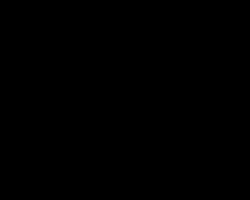
\includegraphics[scale=0.4]{BlobAnalysis/img/memory_0_0}} &
  50000 & 
  6250 & 
  0 \\
  \raisebox{1ex - \height}{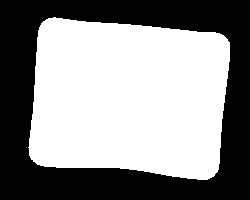
\includegraphics[scale=0.4]{BlobAnalysis/img/memory_1_163}} & 
  50000 & 
  6250 & 
  978 \\
  \raisebox{1ex - \height}{
\includegraphics[scale=0.4]{BlobAnalysis/img/memory_2_1046}} & 
  50000 & 
  6250 & 
  6276 \\ 
  \raisebox{1ex - \height}{
\includegraphics[scale=0.4]{BlobAnalysis/img/memory_3_12517}} & 
  50000 & 
  6250 & 
  75102  \\ 
\end{tabular}
\caption{Number of bytes consumed by different region representations.}
\label{tab:RegionRepresentationMemory}
\end{table}

\subsubsection{Region Dimensions}

\paragraph*{}
In our reference implementation, \studio, regions are represented using the run-length encoding described above, with one slight extension: each region stores two additional integers representing its reference dimensions: width and height.

\paragraph*{}
These are usually the dimensions of image the region was extracted from and serve two purposes. For one thing, they allow meaningful display of a region in the context of image it refers to; for other thing - they conveniently allow to define a complement of a region. Formally, the finite dimensions of the region space allows to distinguish between three types of pixels: set, unset and undefined (outside the region dimensions), i.e. corresponding to undefined image pixels that we have no information about.

\newarray\regionDimensions
\readarray{regionDimensions}{%
0 & 0 & 0 & 0 & 0 & 0 & 0 &%
0 & 1 & 1 & 1 & 0 & 0 & 0 &%
1 & 1 & 1 & 1 & 0 & 0 & 0 &%
0 & 0 & 1 & 0 & 0 & 0 & 0 &%
0 & 0 & 0 & 0 & 0 & 0 & 0}

\dataheight=\gridwidth

\begin{figure}[h!]
\centering

\begin{tikzpicture}[scale=0.40]\drawslabs{regionDimensions}\end{tikzpicture}
\caption{Region of dimensions: 7 (width), 5 (height)}
\label{tab:RegionDimensions}
\end{figure}
\pgfmathtruncatemacro{\gridwidth}{7}
\pgfmathtruncatemacro{\gridheight}{5}

\section{Elementary Operators}

\paragraph*{}
In this section we will introduce six elementary operations that can be performed on regions. Four of them refer to the set nature of regions, two further are defined in relation to its spatial properties. 

\paragraph*{}
In the next section we will use these building blocks to define powerful transformations from the field of Mathematical Morphology.

\subsection{Set Operators}

\paragraph*{}
Applicability of basic set operators to region processing follows directly from the definition of region. 

\subsubsection{Union}

\paragraph*{}
Union of two regions is a region containing the pixels belonging to either, or both of the input regions, as demonstrated in \reftab{RegionUnion}.

\newarray\unionInputA
\readarray{unionInputA}{%
0 & 0 & 0 & 0 & 0 & 0 & 0 &%
0 & 0 & 1 & 1 & 1 & 1 & 0 &%
0 & 0 & 1 & 1 & 0 & 0 & 0 &%
0 & 0 & 1 & 1 & 0 & 0 & 0 &%
0 & 0 & 0 & 0 & 0 & 0 & 0}

\newarray\unionInputB
\readarray{unionInputB}{%
0 & 0 & 0 & 0 & 0 & 0 & 0 &%
0 & 0 & 0 & 1 & 1 & 1 & 0 &%
0 & 0 & 0 & 0 & 0 & 1 & 0 &%
0 & 0 & 0 & 0 & 0 & 1 & 0 &%
0 & 0 & 0 & 0 & 0 & 0 & 0}

\newarray\unionResult
\readarray{unionResult}{%
0 & 0 & 0 & 0 & 0 & 0 & 0 &%
0 & 0 & 1 & 1 & 1 & 1 & 0 &%
0 & 0 & 1 & 1 & 0 & 1 & 0 &%
0 & 0 & 1 & 1 & 0 & 1 & 0 &%
0 & 0 & 0 & 0 & 0 & 0 & 0}

\dataheight=\gridwidth

\begin{table}[h]
\centering
\tabular{c c c}

\begin{tikzpicture}[scale=0.40]\drawslabs{unionInputA}\end{tikzpicture} &
\begin{tikzpicture}[scale=0.40]\drawslabs{unionInputB}\end{tikzpicture} &
\begin{tikzpicture}[scale=0.40]\drawslabs{unionResult}\end{tikzpicture} 

\\

$A$ &
$B$ &
$A \cup B$

\endtabular
\caption{Union of two regions}
\label{tab:RegionUnion}
\end{table}


\subsubsection{Intersection}

\paragraph*{}
Similarily, intersection of two regions is a region containing the pixels belonging to both of the input regions, as demonstrated in \reftab{RegionIntersection}.

\newarray\intersectionInputA
\readarray{intersectionInputA}{%
0 & 0 & 0 & 0 & 0 & 0 & 0 &%
0 & 0 & 1 & 1 & 1 & 1 & 0 &%
0 & 0 & 1 & 1 & 0 & 0 & 0 &%
0 & 0 & 1 & 1 & 0 & 0 & 0 &%
0 & 0 & 0 & 0 & 0 & 0 & 0}

\newarray\intersectionInputB
\readarray{intersectionInputB}{%
0 & 0 & 0 & 0 & 0 & 0 & 0 &%
0 & 0 & 0 & 1 & 1 & 1 & 0 &%
0 & 0 & 0 & 0 & 0 & 1 & 0 &%
0 & 0 & 0 & 0 & 0 & 1 & 0 &%
0 & 0 & 0 & 0 & 0 & 0 & 0}

\newarray\intersectionResult
\readarray{intersectionResult}{%
0 & 0 & 0 & 0 & 0 & 0 & 0 &%
0 & 0 & 0 & 1 & 1 & 0 & 0 &%
0 & 0 & 0 & 0 & 0 & 0 & 0 &%
0 & 0 & 0 & 0 & 0 & 0 & 0 &%
0 & 0 & 0 & 0 & 0 & 0 & 0}

\dataheight=\gridwidth

\begin{table}[h]
\centering
\tabular{c c c}

\begin{tikzpicture}[scale=0.40]\drawslabs{intersectionInputA}\end{tikzpicture} &
\begin{tikzpicture}[scale=0.40]\drawslabs{intersectionInputB}\end{tikzpicture} &
\begin{tikzpicture}[scale=0.40]\drawslabs{intersectionResult}\end{tikzpicture} 

\\

$A$ &
$B$ &
$A \cap B$

\endtabular
\caption{Intersection of two regions}
\label{tab:RegionIntersection}
\end{table}


\subsubsection{Difference}

\paragraph*{}
Last binary operation in this group is difference, yielding the pixels belonging to first region, but not to the second region. Thus, this operation is not commutative, contrary to intersection and union. 

\newarray\differenceInputA
\readarray{differenceInputA}{%
0 & 0 & 0 & 0 & 0 & 0 & 0 &%
0 & 0 & 1 & 1 & 1 & 1 & 0 &%
0 & 0 & 1 & 1 & 0 & 0 & 0 &%
0 & 0 & 1 & 1 & 0 & 0 & 0 &%
0 & 0 & 0 & 0 & 0 & 0 & 0}

\newarray\differenceInputB
\readarray{differenceInputB}{%
0 & 0 & 0 & 0 & 0 & 0 & 0 &%
0 & 0 & 0 & 1 & 1 & 1 & 0 &%
0 & 0 & 0 & 0 & 0 & 1 & 0 &%
0 & 0 & 0 & 0 & 0 & 1 & 0 &%
0 & 0 & 0 & 0 & 0 & 0 & 0}

\newarray\differenceResult
\readarray{differenceResult}{%
0 & 0 & 0 & 0 & 0 & 0 & 0 &%
0 & 0 & 1 & 0 & 0 & 0 & 0 &%
0 & 0 & 1 & 1 & 0 & 0 & 0 &%
0 & 0 & 1 & 1 & 0 & 0 & 0 &%
0 & 0 & 0 & 0 & 0 & 0 & 0}

\dataheight=\gridwidth

\begin{table}[h]
\centering
\tabular{c c c}

\begin{tikzpicture}[scale=0.40]\drawslabs{differenceInputA}\end{tikzpicture} &
\begin{tikzpicture}[scale=0.40]\drawslabs{differenceInputB}\end{tikzpicture} &
\begin{tikzpicture}[scale=0.40]\drawslabs{differenceResult}\end{tikzpicture} 

\\

$A$ &
$B$ &
$A \setminus B$

\endtabular
\caption{Difference of two regions}
\label{tab:RegionDifference}
\end{table}

\subsubsection{Complement}

\paragraph*{}
The only unary set operator, complement, is also applicable to region; however industrial implementations differ in its interpretation. We will follow the way of our reference implementation, where complement is easy to define as each region stores the dimensions of its finite reference space.

\newarray\complementInput
\readarray{complementInput}{%
0 & 0 & 0 & 0 & 0 & 0 & 0 &%
0 & 0 & 1 & 1 & 1 & 1 & 0 &%
0 & 0 & 1 & 1 & 0 & 0 & 0 &%
0 & 0 & 1 & 1 & 0 & 0 & 0 &%
0 & 0 & 0 & 0 & 0 & 0 & 0}

\newarray\complementResult
\readarray{complementResult}{%
1 & 1 & 1 & 1 & 1 & 1 & 1 &%
1 & 1 & 0 & 0 & 0 & 0 & 1 &%
1 & 1 & 0 & 0 & 1 & 1 & 1 &%
1 & 1 & 0 & 0 & 1 & 1 & 1 &%
1 & 1 & 1 & 1 & 1 & 1 & 1}

\dataheight=\gridwidth

\begin{table}[h!]
\centering
\tabular{c c}

\begin{tikzpicture}[scale=0.40]\drawslabs{complementInput}\end{tikzpicture} &
\begin{tikzpicture}[scale=0.40]\drawslabs{complementResult}\end{tikzpicture} 

\\

$A$ &
$A^{\complement}$

\endtabular
\caption{Complement of a region}
\label{tab:RegionComplement}
\end{table}


\subsection{Spatial Operators}

\paragraph*{} 
Two further operators refer to spatial properties of region. Naturally, there are far more spatial operators than can be defined for region; for now we introduce only two that are neccessary to define morphological operators discussed in the next section.

\subsubsection{Translation}

\paragraph*{}
Translation of a region shifts its pixel coordinates by integer vector.

\newarray\translationInput
\readarray{translationInput}{%
0 & 0 & 0 & 0 & 0 & 0 & 0 &%
0 & 0 & 1 & 1 & 1 & 1 & 0 &%
0 & 0 & 1 & 1 & 0 & 0 & 0 &%
0 & 0 & 1 & 1 & 0 & 0 & 0 &%
0 & 0 & 0 & 0 & 0 & 0 & 0}

\newarray\translationResult
\readarray{translationResult}{%
0 & 0 & 0 & 0 & 0 & 0 & 0 &%
0 & 0 & 0 & 0 & 0 & 0 & 0 &%
1 & 1 & 1 & 1 & 0 & 0 & 0 &%
1 & 1 & 0 & 0 & 0 & 0 & 0 &%
1 & 1 & 0 & 0 & 0 & 0 & 0}

\dataheight=\gridwidth

\begin{table}[h!]
\centering
\tabular{c c}

\begin{tikzpicture}[scale=0.40]\drawslabs{translationInput}\end{tikzpicture} &
\begin{tikzpicture}[scale=0.40]\drawslabs{translationResult}\end{tikzpicture} 

\\

$A$ &
$Translate(A, v)$

\endtabular
\caption{Translation of a region by vector -2,1.}
\label{tab:RegionTranslation}
\end{table}

\subsection{Reflection}

\paragraph*{}
Reflection mirrors a region over a location (origin). This operation will be particulary useful for processing morphological kernels, which we will discuss in the next section.

\newarray\reflectionInput
\readarray{reflectionInput}{%
0 & 0 & 0 & 0 & 0 & 0 & 0 &%
0 & 0 & 1 & 0 & 0 & 0 & 0 &%
0 & 0 & 1 & 2 & 0 & 0 & 0 &%
0 & 0 & 0 & 0 & 0 & 0 & 0 &%
0 & 0 & 0 & 0 & 0 & 0 & 0}

\newarray\reflectionResult
\readarray{reflectionResult}{%
0 & 0 & 0 & 0 & 0 & 0 & 0 &%
0 & 0 & 0 & 0 & 0 & 0 & 0 &%
0 & 0 & 0 & 2 & 1 & 0 & 0 &%
0 & 0 & 0 & 0 & 1 & 0 & 0 &%
0 & 0 & 0 & 0 & 0 & 0 & 0}

\begin{table}[h!]
	\centering
	\tabular{c c}
		\begin{tikzpicture}[scale=0.40]\drawslabs{reflectionInput}\end{tikzpicture} &
		\begin{tikzpicture}[scale=0.40]\drawslabs{reflectionResult}\end{tikzpicture} 
		\\
		$A$ &
		$Reflect(A, org)$
	\endtabular
	\caption{Reflection of a region, its origin marked with a black square.}
	\label{tab:RegionReflection}
\end{table}
\section{Mathematical Morphology}

\paragraph*{}
Mathematical Morphology, born in 1960s and rapidly developing ever since, is both a theory and a technique for processing spatial structures. Soille described\cite{Soille03} the field as being \textit{mathematical} in that it is built upon set theory and geometry, and being \textit{morphology}\footnote{From Greek \textit{morphe} meaning form.} in that it aims at analyzing the shape of objects.

\paragraph*{}
In most general case, Mathematical Morphology applies to any complete lattice. We will concentrate on its application to region processing. In this context Mathematical Morphology can be looked at as a set of techniques that alter a region by probing it with another shape called kernel or structuring element.

\subsection{Kernel}

\paragraph*{}
Kernel in Mathematical Morphology is a shape that is repeatedly aligned at each position within the dimensions of the region being processed. At each such alignment the operator verifies how the aligned kernel fits in the region (e.g. if the kernel is contained in the region in its entirety) and depending on the results includes the location in the results or not.

\paragraph*{}
As kernel is pixel-precise binary shape itself, it can be represented as a region together with integer coordinates of its origin. Specifying the origin is important, as it is the position that will be aligned against the region being processed.

\gridDimensions{5}{5}

\newarray\kernelA
\readarray{kernelA}{%
0 & 0 & 0 & 0 & 0 &%
0 & 1 & 1 & 1 & 0 &%
0 & 1 & 2 & 1 & 0 &%
0 & 1 & 1 & 1 & 0 &%
0 & 0 & 0 & 0 & 0}

\newarray\kernelB
\readarray{kernelB}{%
0 & 0 & 0 & 0 & 0 &%
0 & 0 & 1 & 0 & 0 &%
0 & 1 & 2 & 1 & 0 &%
0 & 0 & 1 & 0 & 0 &%
0 & 0 & 0 & 0 & 0}

\newarray\kernelC
\readarray{kernelC}{%
0 & 0 & 0 & 0 & 0 &%
0 & 0 & 0 & 0 & 0 &%
0 & 0 & 2 & 1 & 0 &%
0 & 0 & 1 & 0 & 0 &%
0 & 0 & 0 & 0 & 0}


\begin{table}[h!]
\centering
\tabular{c c c}


\gridDimensions{5}{5}\begin{tikzpicture}[scale=0.40]\drawslabs{kernelA}\end{tikzpicture} &
\gridDimensions{5}{5}\begin{tikzpicture}[scale=0.40]\drawslabs{kernelB}\end{tikzpicture} &
\gridDimensions{5}{5}\begin{tikzpicture}[scale=0.40]\drawslabs{kernelC}\end{tikzpicture} 

\endtabular
\caption{Example kernels for morphological operations.}
\label{tab:MorphologyKernels}
\end{table}


\subsection{Dilation}

\paragraph*{}
First morphological operation that we are going to discuss is dilation. In this operator the kernel aligned at each position within the region dimensions needs to overlap with at least one pixel of the input region to include this position in the result:

\[
	Dilate(R,K) = \{[p_x,p_y] | R \cap Translate(K, [p_x,p_y]) \neq \emptyset \}
\] 

\newarray\dilationInput
\readarray{dilationInput}{%
0 & 0 & 0 & 0 & 0 & 0 & 0 &%
0 & 0 & 1 & 0 & 0 & 0 & 0 &%
0 & 1 & 0 & 1 & 1 & 1 & 0 &%
0 & 1 & 0 & 0 & 0 & 1 & 0 &%
0 & 0 & 0 & 0 & 0 & 0 & 0}

\newarray\dilationKernel
\readarray{dilationKernel}{%
0 & 0 & 0 & 0 & 0 &%
0 & 0 & 1 & 0 & 0 &%
0 & 1 & 2 & 1 & 0 &%
0 & 0 & 1 & 0 & 0 &%
0 & 0 & 0 & 0 & 0}

\newarray\dilationResult
\readarray{dilationResult}{%
0 & 0 & 1 & 0 & 0 & 0 & 0 &%
0 & 1 & 1 & 1 & 1 & 1 & 0 &%
1 & 1 & 1 & 1 & 1 & 1 & 1 &%
1 & 1 & 1 & 1 & 1 & 1 & 1 &%
0 & 1 & 0 & 0 & 0 & 1 & 0}

\begin{table}[h]
\centering
\tabular{c c c}

\gridDimensions{7}{5}\begin{tikzpicture}[scale=0.40]\drawslabs{dilationInput}\end{tikzpicture} &
\gridDimensions{5}{5}\begin{tikzpicture}[scale=0.40]\drawslabs{dilationKernel}\end{tikzpicture} &
\gridDimensions{7}{5}\begin{tikzpicture}[scale=0.40]\drawslabs{dilationResult}\end{tikzpicture} 

\\

$R$ &
$K$ &
$Dilate(R,K)$

\endtabular
\caption{Dilation of a region}
\label{tab:RegionDilation}
\end{table}

\paragraph*{}
If we decompose the kernel into its individual pixels we may observe that each such pixel $[k_x, k_y] \in K$ contributes a copy of the region translated by $[-k_x, -k_y]$ into the result. Therefore we may also define the dilation operator as follows:
\[
	Dilate(R,K) = \bigcup_{[k_x, k_y] \in K} Translate(R, [-k_x, -k_y])
\]

\paragraph*{}
Dilation effectively expands the region, the magnitude and direction of the expansion depending on the kernel being used. The operator is commonly used to join disconnected components of a region. Dilating a region by circular kernel of radius $r$ will expand the region uniformly in each direction up to distance of $r$ pixels, effectively joining region components separated by less than $2r$ pixels. One possible application is demonstrated in \reffig{DilationAppliedToFuses}.

\paragraph*{}
In this example we process a region representing metal parts of two fuses. As one of the fuses is burned out, the region contains three connected components. To split it into two connected components, each representing an individual fuse, we may perform the dilation before extracting the region components and intersect the resulting regions with the original one to preserve their original shape.

\begin{figure}
    \begin{subfigure}[b]{\basicWidth}
            \centering
            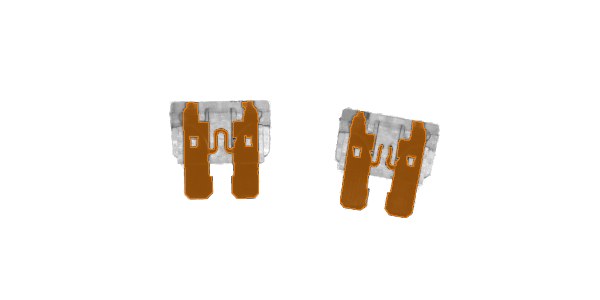
\includegraphics[width=\linewidth]{BlobAnalysis/img/fuses_region}
            \caption{}
    \end{subfigure}%
    ~
    \begin{subfigure}[b]{\basicWidth}
            \centering
            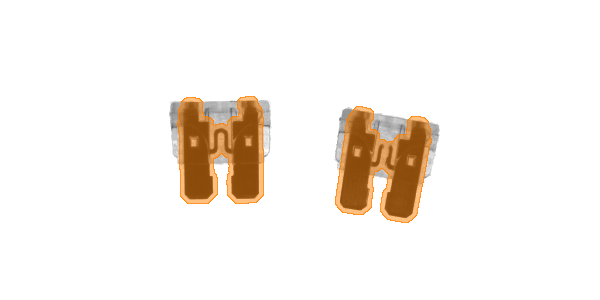
\includegraphics[width=\linewidth]{BlobAnalysis/img/fuses_dilated}
            \caption{}
    \end{subfigure}

    \begin{subfigure}[b]{\basicWidth}
            \centering
            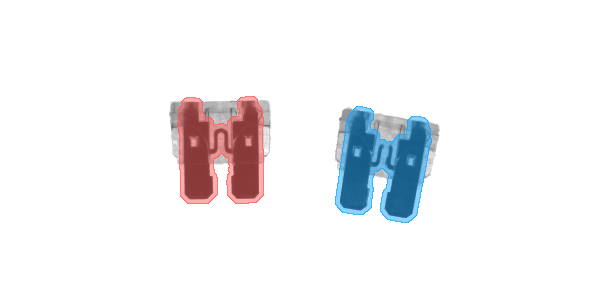
\includegraphics[width=\linewidth]{BlobAnalysis/img/fuses_dilated_blobs}
            \caption{}
    \end{subfigure}%
    ~
    \begin{subfigure}[b]{\basicWidth}
            \centering
            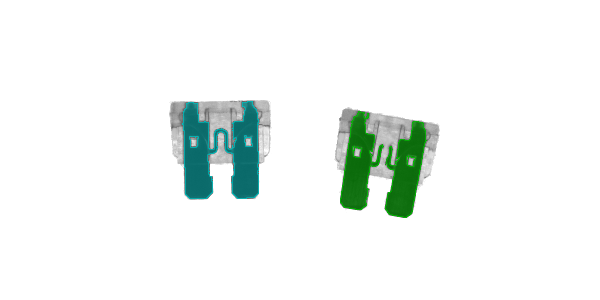
\includegraphics[width=\linewidth]{BlobAnalysis/img/fuses_components}
            \caption{}
    \end{subfigure}
    
    \caption{Dilation, extraction of connected components and intersection applied to split a region representing metal parts of the fuses (a) into components representing individual fuses (d).}
    \label{fig:DilationAppliedToFuses}
\end{figure}

\subsection{Erosion}

\paragraph*{}
Erosion is a shrinking counterpart of dilation. This operator requires that the aligned kernel is fully contained in the region being processed:

\[
	Erode(R,K) = \{[p_x,p_y] | Translate(K, [p_x,p_y]) \subseteq R \}
\] 

\newarray\erosionInput
\readarray{erosionInput}{%
0 & 0 & 1 & 0 & 0 & 0 & 0 &%
0 & 1 & 1 & 1 & 1 & 1 & 0 &%
1 & 1 & 1 & 1 & 1 & 1 & 1 &%
1 & 1 & 1 & 1 & 1 & 1 & 1 &%
0 & 1 & 0 & 0 & 0 & 1 & 0}

\newarray\erosionKernel
\readarray{erosionKernel}{%
0 & 0 & 0 & 0 & 0 &%
0 & 0 & 1 & 0 & 0 &%
0 & 1 & 2 & 1 & 0 &%
0 & 0 & 1 & 0 & 0 &%
0 & 0 & 0 & 0 & 0}

\newarray\erosionResult
\readarray{erosionResult}{%
0 & 0 & 0 & 0 & 0 & 0 & 0 &%
0 & 0 & 1 & 0 & 0 & 0 & 0 &%
0 & 1 & 1 & 1 & 1 & 1 & 0 &%
0 & 1 & 0 & 0 & 0 & 1 & 0 &%
0 & 0 & 0 & 0 & 0 & 0 & 0}

\begin{table}[h]
\centering
\tabular{c c c}

\gridDimensions{7}{5}\begin{tikzpicture}[scale=0.40]\drawslabs{erosionInput}\end{tikzpicture} &
\gridDimensions{5}{5}\begin{tikzpicture}[scale=0.40]\drawslabs{erosionKernel}\end{tikzpicture} &
\gridDimensions{7}{5}\begin{tikzpicture}[scale=0.40]\drawslabs{erosionResult}\end{tikzpicture} 

\\

$R$ &
$K$ &
$Erode(R,K)$

\endtabular
\caption{Erosion of a region}
\label{tab:RegionErosion}
\end{table}

\paragraph*{}
Similarly to dilation, we may also formulate erosion in terms of kernel decomposition. In this case each pixel of the kernel $[k_x, k_y] \in K$ also contributes the shifted copy of a region, but a position must be contained in all such contributions to be included in the results:
\[
	Erode(R,K) = \bigcap_{[k_x, k_y] \in K} Translate(R, [-k_x, -k_y])
\]

\paragraph*{}
The operations of dilation and erosion are closely related, but it is important to note that they are not inverse\footnote{Actually neither of these operation has an inverse, as such operation would have to magically guess where the lone pixels lost in erosion or holes filled in dilation were located.} of each other, i.e., erosion of a region does not necessarily \textit{cancel out} previously applied dilation; counterexample being presented in \reftab{RegionDilation} and \reftab{RegionErosion}. Quite contrary, consecutive application of dilation and erosion is extremely useful operation and will be discussed soon.

\paragraph*{}
Although dilation is not an inverse of erosion, another relation between the operations holds - they are duals of each other, meaning that dilation of a region is equivalent to erosion of its background (complement), and conversely.

\[
	Erode(R, K) = Dilate(R^{\complement}, K)^{\complement}
\]

\subsection{Closing}

\paragraph*{}
Before we define the next operator, let us get back for a moment to the dilation operator. As we remember, dilation expands the region in the way defined by the structuring element. It is worth noting that during this expansion small holes and region cavities may get completely filled in. This effect is worth attention as filling gaps of a region\footnote{Which could be introduced for instance by local glare of the lightning affecting the results of thresholding.} is a common need in industrial inspection.

\paragraph*{}
Unfortunately, dilation does not address this need precisely - the missing parts gets filled in, but also the region boundaries are expanded. It would be more convenient to have an operator that avoids the second effect while keeping the first.

\paragraph*{}
The closing operator addresses this need by dilating the region and eroding it right after that:
\[
	Close(R,K) = Erode(Dilate(R, K), Reflect(K))
\] 

\paragraph*{}
Initial dilation fills in the region gaps and the succeeding erosion brings the expanded region back to its original dimensions (but does not restore the gaps that were completely filled in). 

\paragraph*{}
It is worth noting that we use the reflected kernel for the second operation - if we recall that dilation may be formulated as a union of translations corresponding to individual pixels of the kernel ($\bigcup_{[k_x, k_y] \in K} Translate(R, [-k_x, -k_y])$), it is clear that we need to use the opposite translations to keep the region in its position.

\newarray\closingInput
\readarray{closingInput}{%
0 & 0 & 0 & 0 & 0 & 0 & 0 &%
0 & 0 & 1 & 0 & 0 & 0 & 0 &%
0 & 1 & 0 & 1 & 1 & 1 & 0 &%
0 & 1 & 0 & 0 & 0 & 1 & 0 &%
0 & 0 & 0 & 0 & 0 & 0 & 0}

\newarray\closingKernel
\readarray{closingKernel}{%
0 & 0 & 0 & 0 & 0 &%
0 & 0 & 1 & 0 & 0 &%
0 & 1 & 2 & 1 & 0 &%
0 & 0 & 1 & 0 & 0 &%
0 & 0 & 0 & 0 & 0}

\newarray\closingResult
\readarray{closingResult}{%
0 & 0 & 0 & 0 & 0 & 0 & 0 &%
0 & 0 & 1 & 0 & 0 & 0 & 0 &%
0 & 1 & 1 & 1 & 1 & 1 & 0 &%
0 & 1 & 0 & 0 & 0 & 1 & 0 &%
0 & 0 & 0 & 0 & 0 & 0 & 0}

\begin{table}[h]
\centering
\tabular{c c c}

\gridDimensions{7}{5}\begin{tikzpicture}[scale=0.40]\drawslabs{closingInput}\end{tikzpicture} &
\gridDimensions{5}{5}\begin{tikzpicture}[scale=0.40]\drawslabs{closingKernel}\end{tikzpicture} &
\gridDimensions{7}{5}\begin{tikzpicture}[scale=0.40]\drawslabs{closingResult}\end{tikzpicture} 

\\

$R$ &
$K$ &
$Close(R,K)$

\endtabular
\caption{Closing of a region}
\label{tab:RegionClosing}
\end{table}

\paragraph*{}
Closing is commonly applied whenever the extracted region contains gaps or cavities that should be filled in, an example of such application is demonstrated in \reffig{RegionClosingApplied}.

\twoFigures
{BlobAnalysis/img/morphology_close_before}
{BlobAnalysis/img/morphology_close_after}
{Closing operator used to fill gaps in a region.}
{RegionClosingApplied}
{\basicWidth}

\subsection{Opening}

\paragraph*{}
Another useful morphological operator is obtained by interchanging the order of operators that closing is composed of. The opening operator firstly erode a region and then dilates the result:

\[
	Open(R,K) = Dilate(Erode(R, K), Reflect(K))
\] 

\paragraph*{}
The effect of such composition is dual to the closing operator that we recently discussed. The initial erosion shrinks the region removing its isolated pixels and small branches, while the successive dilation brings it back to original dimensions, but cannot restore the parts that vanished completely during erosion.

\newarray\openingInput
\readarray{openingInput}{%
0 & 0 & 0 & 0 & 0 & 1 & 0 &%
0 & 0 & 1 & 0 & 0 & 0 & 0 &%
0 & 1 & 1 & 1 & 1 & 0 & 1 &%
1 & 1 & 1 & 0 & 0 & 0 & 0 &%
0 & 1 & 0 & 0 & 0 & 0 & 0}

\newarray\openingKernel
\readarray{openingKernel}{%
0 & 0 & 0 & 0 & 0 &%
0 & 0 & 1 & 0 & 0 &%
0 & 1 & 2 & 1 & 0 &%
0 & 0 & 1 & 0 & 0 &%
0 & 0 & 0 & 0 & 0}

\newarray\openingResult
\readarray{openingResult}{%
0 & 0 & 0 & 0 & 0 & 0 & 0 &%
0 & 0 & 1 & 0 & 0 & 0 & 0 &%
0 & 1 & 1 & 1 & 0 & 0 & 0 &%
1 & 1 & 1 & 0 & 0 & 0 & 0 &%
0 & 1 & 0 & 0 & 0 & 0 & 0}

\begin{table}[h]
\centering
\tabular{c c c}

\gridDimensions{7}{5}\begin{tikzpicture}[scale=0.40]\drawslabs{openingInput}\end{tikzpicture} &
\gridDimensions{5}{5}\begin{tikzpicture}[scale=0.40]\drawslabs{openingKernel}\end{tikzpicture} &
\gridDimensions{7}{5}\begin{tikzpicture}[scale=0.40]\drawslabs{openingResult}\end{tikzpicture} 

\\

$R$ &
$K$ &
$Open(R,K)$

\endtabular
\caption{Opening of a region}
\label{tab:RegionOpening}
\end{table}

\paragraph*{}
The opening operator may be applied to remove salt noise in the region or to eliminate its thin parts. Opening a region using a circular kernel of radius $r$ will remove all segments of the region that have less than $2r$ pixels in width (and keep the other parts intact). An example application is demonstrated in \reffig{RegionOpeningApplied}.

\twoFigures
{BlobAnalysis/img/morphology_open_before}
{BlobAnalysis/img/morphology_open_after}
{Opening operator used to determine excessively wide section of the rubber band.}
{RegionOpeningApplied}
{\basicWidth}

\begin{refImpl}
Basic morphological operators described in this section are available as \studio \,filters:
\begin{itemize}
    \item \filter{DilateRegion}{RegionMorphology}, \filter{DilateRegion\_AnyKernel}{RegionMorphology}
    \item \filter{ErodeRegion}{RegionMorphology}, \filter{ErodeRegion\_AnyKernel}{RegionMorphology}
    \item \filter{CloseRegion}{RegionMorphology}, \filter{CloseRegion\_AnyKernel}{RegionMorphology}
    \item \filter{OpenRegion}{RegionMorphology}, \filter{OpenRegion\_AnyKernel}{RegionMorphology}
\end{itemize}
The filters with \textit{\_AnyKernel} suffix allow to perform the operation using arbitrary kernel, while their counterparts allow to choose from a set of predefined, hard-coded kernels.
\end{refImpl}
%\section{Hit-and-Miss and Skeletons [under construction]}

\paragraph*{}
In the previous section we have seen a set of morphological operators, all of which accept a single binary kernel which is used to probe and transform the given region. In this section we will introduce an operation that effectively uses two disjoint kernels to probe the region being processed and explore new possibilities opened by such extension.

\subsection{Hit-and-Miss}

\paragraph*{}
Hit-and-Miss (also called \textit{Hit-or-Miss}) is essentially a Template Matching operator built upon morphological processing. Here the template to be matched is modeled using two disjoint kernels. First kernel, called \textit{Hit Kernel} or \textit{Foreground Kernel} represents the pixels that have to belong to the region at each position while the second kernel (\textit{Miss Kernel}, \textit{Background Kernel}) represents the pixels that must not belong to the region (i.e. must belong to its background).

\paragraph*{}
For brevity we depict each pair of kernels (or each \textit{composite} kernel) on a single picture, using blue color for Hit Kernel and red color for Miss Kernel, as demonstrated in \reftab{CompositeKernel}.

\gridDimensions{5}{5}

\newarray\compositeKernel
\readarray{compositeKernel}{%
0 & 0 & 0 & 0 & 0 &%
0 & 3 & 3 & 3 & 0 &%
0 & 3 & 2 & 3 & 0 &%
0 & 3 & 3 & 3 & 0 &%
0 & 0 & 0 & 0 & 0}


\begin{table}[h!]
\centering
\tabular{c c c}

\gridDimensions{5}{5}\begin{tikzpicture}[scale=0.40]\drawslabs{compositeKernel}\end{tikzpicture}

\endtabular
\caption{Composite kernel for Hit-or-Miss transform matching isolated region pixels.}
\label{tab:CompositeKernel}
\end{table}

\paragraph*{}
Hit-and-Miss operator aligns such kernel at each location within the region dimensions and includes this position in the result only if both foreground and background configuration is correctly matched:

\[
\begin{array}{l}
HitAndMiss(R,K_{Hit},K_{Miss}) =  \{ [p_x,p_y] | \\
\quad Translate(K_{Hit}, [p_x,p_y]) \subseteq R \bigwedge 
 Translate(K_{Miss}, [p_x,p_y]) \subseteq R^{\complement} \} 

\end{array}
\]


\newarray\hitAndMissInput
\readarray{hitAndMissInput}{%
0 & 0 & 0 & 0 & 0 & 0 & 0 &%
0 & 1 & 1 & 0 & 0 & 1 & 0 &%
0 & 0 & 1 & 1 & 0 & 0 & 0 &%
0 & 1 & 0 & 1 & 1 & 1 & 0 &%
0 & 0 & 0 & 0 & 0 & 0 & 0}

\newarray\hitAndMissKernel
\readarray{hitAndMissKernel}{%
0 & 0 & 0 & 0 & 0 &%
0 & 0 & 3 & 0 & 0 &%
0 & 3 & 2 & 3 & 0 &%
0 & 0 & 3 & 0 & 0 &%
0 & 0 & 0 & 0 & 0}

\newarray\hitAndMissResult
\readarray{hitAndMissResult}{%
0 & 0 & 0 & 0 & 0 & 0 & 0 &%
0 & 0 & 0 & 0 & 0 & 1 & 0 &%
0 & 0 & 0 & 0 & 0 & 0 & 0 &%
0 & 1 & 0 & 0 & 0 & 0 & 0 &%
0 & 0 & 0 & 0 & 0 & 0 & 0}

\begin{table}[h]
\centering
\tabular{c c c}

\gridDimensions{7}{5}\begin{tikzpicture}[scale=0.40]\drawslabs{hitAndMissInput}\end{tikzpicture} &
\gridDimensions{5}{5}\begin{tikzpicture}[scale=0.40]\drawslabs{hitAndMissKernel}\end{tikzpicture} &
\gridDimensions{7}{5}\begin{tikzpicture}[scale=0.40]\drawslabs{hitAndMissResult}\end{tikzpicture} 

\\

$R$ &
$K = (K_{Hit}, K_{Miss})$ &
$HitAndMiss(R, K)$

\endtabular
\caption{Hit-and-Miss operator finds isolated region pixels.}
\label{tab:HitAndMiss}
\end{table}

\paragraph*{}
If we recall that erosion essentially selects locations where given kernel fits the region pixels we may define Hit-and-Miss as intersection of two erosions:

\[
	HitAndMiss(R, K_{Hit}, K_{Miss}) = Erode(R, K_{Hit}) \cap Erode(R^{\complement}, K_{Miss})
\]

\paragraph*{}
Alternatively, we may use an erosion to determine the set of locations where the foreground condition is met, and a dilation to determine the set of locations where the background condition is violated, yielding definition:

\[
	HitAndMiss(R, K_{Hit}, K_{Miss}) = Erode(R, K_{Hit}) \setminus Dilate(R, K_{Miss})
\]

\paragraph*{}
Hit-and-Miss operator is often applied repeatedly using a set of kernels, e.g. representing rotations of the pattern that is to be identified. \reftab{RegionEndpoints} demonstrates how Hit-and-Miss operator may be applied to find foreground endpoints in a region. Here each of four rotations of the composite kernel is matched individually and their union constitutes the final outcome.

\newarray\regionEndpointsInput
\readarray{regionEndpointsInput}{%
0 & 0 & 0 & 0 & 0 & 0 & 0 &%
0 & 1 & 1 & 1 & 1 & 1 & 0 &%
0 & 0 & 0 & 0 & 0 & 1 & 0 &%
0 & 1 & 0 & 0 & 1 & 1 & 0 &%
0 & 0 & 0 & 0 & 0 & 0 & 0}

\newarray\regionEndpointsKernel
\readarray{regionEndpointsKernel}{%
0 & 0 & 0 & 0 & 0 &%
0 & 0 & 0 & 0 & 0 &%
0 & 3 & 2 & 3 & 0 &%
0 & 0 & 3 & 0 & 0 &%
0 & 0 & 0 & 0 & 0}

\newarray\regionEndpointsResult
\readarray{regionEndpointsResult}{%
0 & 0 & 0 & 0 & 0 & 0 & 0 &%
0 & 1 & 0 & 0 & 0 & 0 & 0 &%
0 & 0 & 0 & 0 & 0 & 0 & 0 &%
0 & 1 & 0 & 0 & 1 & 0 & 0 &%
0 & 0 & 0 & 0 & 0 & 0 & 0}

\begin{table}[h]
\centering
\tabular{c c l}

\gridDimensions{7}{5}\begin{tikzpicture}[scale=0.40]\drawslabs{regionEndpointsInput}\end{tikzpicture} &
\gridDimensions{5}{5}\begin{tikzpicture}[scale=0.40]\drawslabs{regionEndpointsKernel}\end{tikzpicture} &
\gridDimensions{7}{5}\begin{tikzpicture}[scale=0.40]\drawslabs{regionEndpointsResult}\end{tikzpicture} 

\\

$R$ &
$K_{0} = (K_{Hit}, K_{Miss})$ &
$HitAndMiss(R, K_{0})$

\\
& & $\cup HitAndMiss(R, K_{90})$
\\ 
& & $\cup HitAndMiss(R, K_{180})$
\\ 
& & $\cup HitAndMiss(R, K_{270})$
\endtabular
\caption{Foreground endpoints located using Hit-and-Miss operator.}
\label{tab:RegionEndpoints}
\end{table}

\subsection{Thinning}

\paragraph*{}


\subsection{Thickening}

\subsection{Skeletons}

\section{Topology}

\paragraph*{}
We have already seen operations defined in the context of set nature of the region as well as operations concerned with its spatial properties. The last set of transformations that we will discuss is built upon topological concepts such as neighborhood, connectivity or boundaries.

\subsection{Connectivity}

\paragraph*{}
Pixel connectivity defines the conditions in which we say that two pixels are \textit{connected} and as such is a key concept in the context of topological transformations. There is a well known paradox inherently associated with the definition of binary shapes connectivity on square grids\footnote{On triangular grids as well, but not on hexagonal ones.}.

\paragraph*{}
To demonstrate the paradox let us consider a closed not self-intersecting curve. Jordan Curve Theorem (and our common sense) requires that such curve should divide the space in which it lies into exactly two parts - interior and exterior. The paradox of pixel connectivity lies in the fact that this requirement is not met under either of two reasonable definitions of pixel connectivity.

\paragraph*{}
One possible definition of connectivity is 4-connectivity in which a pixel is consider connected to the pixels it shares an edge with, as demonstrated in \reftab{FourConnectivity}. Under this definition the curve on the right splits the space into three, rather than two connected components.

\newarray\fourNeighborhood
\readarray{fourNeighborhood}{%
0 & 0 & 0 & 0 & 0 &%
0 & 0 & 1 & 0 & 0 &%
0 & 1 & 2 & 1 & 0 &%
0 & 0 & 1 & 0 & 0 &%
0 & 0 & 0 & 0 & 0}

\newarray\fourExample
\readarray{fourExample}{%
0 & 0 & 0 & 0 & 0 & 0 & 0 & 0 &%
0 & 1 & 1 & 1 & 1 & 0 & 0 & 0 &%
0 & 1 & 0 & 0 & 1 & 0 & 0 & 0 &%
0 & 1 & 0 & 0 & 1 & 1 & 1 & 0 &%
0 & 1 & 1 & 1 & 0 & 0 & 1 & 0 &%
0 & 0 & 0 & 1 & 0 & 0 & 1 & 0 &%
0 & 0 & 0 & 1 & 1 & 1 & 1 & 0 &%
0 & 0 & 0 & 0 & 0 & 0 & 0 & 0}

\begin{table}[h]
\centering
\tabular{c c}

\gridDimensions{5}{5}\begin{tikzpicture}[scale=0.40]\drawslabs{fourNeighborhood}\end{tikzpicture} &
\gridDimensions{8}{8}\begin{tikzpicture}[scale=0.25]\drawslabs{fourExample}\end{tikzpicture}

\endtabular
\caption{4-connectivity kernel and a curve demonstrating a violation of the Jordan curve property.}
\label{tab:FourConnectivity}
\end{table}

\paragraph*{}
Another option to consider is 8-connectivity in which a pixel is considered connected to the pixels it shares a corner with, as demonstrated in \reftab{EightConnectivity}. Unfortunately in this case it is possible to construct a closed curve that does not split the space at all, i.e. curve the interior of which remains connected to the exterior, as demonstrated on the right.

\newarray\eightNeighborhood
\readarray{eightNeighborhood}{%
0 & 0 & 0 & 0 & 0 &%
0 & 1 & 1 & 1 & 0 &%
0 & 1 & 2 & 1 & 0 &%
0 & 1 & 1 & 1 & 0 &%
0 & 0 & 0 & 0 & 0}

\newarray\eightExample
\readarray{eightExample}{%
0 & 0 & 0 & 0 & 0 & 0 & 0 & 0 &%
0 & 1 & 1 & 1 & 1 & 0 & 0 & 0 &%
0 & 1 & 0 & 0 & 1 & 0 & 0 & 0 &%
0 & 1 & 0 & 0 & 0 & 1 & 1 & 0 &%
0 & 1 & 1 & 0 & 0 & 0 & 1 & 0 &%
0 & 0 & 0 & 1 & 0 & 0 & 1 & 0 &%
0 & 0 & 0 & 1 & 1 & 1 & 1 & 0 &%
0 & 0 & 0 & 0 & 0 & 0 & 0 & 0}

\begin{table}[h]
\centering
\tabular{c c}

\gridDimensions{5}{5}\begin{tikzpicture}[scale=0.40]\drawslabs{eightNeighborhood}\end{tikzpicture} &
\gridDimensions{8}{8}\begin{tikzpicture}[scale=0.25]\drawslabs{eightExample}\end{tikzpicture}

\endtabular
\caption{8-connectivity kernel and a curve demonstrating a violation of the Jordan curve property.}
\label{tab:EightConnectivity}
\end{table}

\paragraph*{}
Rosenfeld proposed\cite{Rosenfeld70} to address this problem by using different connectivities for foreground and background, which yields two feasible configurations:
\begin{itemize}
	\item 4-connectivity for foreground, 8-connectivity for background
	\item 8-connectivity for foreground, 4-connectivity for background
\end{itemize}
From now on we will use the terms 4-connectivity and 8-connectivity in the context of foreground connectivity, quietly assuming that the other type of connectivity is used for background.

\subsection{Connected Components}

\paragraph*{}
The necessity of splitting a region into its connected components (also referred to as \textit{blobs}) occurs naturally whenever the image contains a number of objects and single thresholding is used to extract one region collectively representing all of them. We have already seen an example of such proceeding in \reffig{DilationAppliedToFuses}. 

\paragraph*{}
Let us begin with a remark on more general problem of computing the connected components of any graph. In such case there are two ways one can follow: we can either traverse the components of the graph one component at a time (using either breadth-first or depth-first search) or go through the edges of the graph maintaining and updating a Union-Find structure representing our knowledge of connected components in graph (i.e. determining all connected components at the same time).

\paragraph*{}
As we represent regions as lists of pixel runs, the problem boils down to identification of the connected components of a set of pixel runs. Both of the approaches described above can be adapted to do so. Careful implementation of the DFS/BFS based technique performs in $O(R)$ time complexity, while the Union-Find based solution works in $O(R\log^{*}R)$.

\paragraph*{}
In either case to achieve target complexity it is crucial to carefully go through the region point runs determining the neighbors of each run (either building graph to which we will apply DFS/BFS or updating the Union-Find structure). Splitting the list of point runs into separate lists for each row within the region dimensions allow to do that in $O(R)$ time.

\subsection{Region Holes}

\paragraph*{}
The intuitive concept of a region hole may be formalized as follows:

\begin{description}
	\item[Region hole] is a connected component of region complement that is not adjacent to the boundaries of the region dimensions.
\end{description}

\paragraph*{}
An algorithm for extraction of the region holes may be derived straight from this definition. The one detail we should remember about is to use the background connectivity when computing the connected components of the region complement, as discussed before. 

\begin{refImpl}
\studio filter \filter{SplitRegionIntoBlobs}{RegionGlobalTransforms} extracts an array of region connected components while \filter{RegionHoles}{RegionFeatures} returns an array of region holes computed as decribed above.
\end{refImpl}
\section{Features}

\paragraph*{}
Once we have acquired a region that accurately represents the object that we intend to analyze, we may proceed to extraction of the region features. Features of two-dimensional shapes (discreet regions as well as continuous polygons) may be organized into two groups: statistical and geometrical.

\paragraph*{}
\textbf{Statistical features} of a shape are built upon statistical concepts such as mean or variance and may be computed directly from the coordinates of region pixels or polygon points, disregarding any spatial relations between them. Statistical shape features include, among others, its area, mass center and orientation (i.e. direction of the principal axis of inertia).

\paragraph*{}
\textbf{Geometrical features} are defined in the context of spatial relations between pixels or points contained in the shape. Some of the features, such as circularity factor, are numeric properties, others, such as smallest bounding circle, take form of geometric primitives.

\paragraph*{}
Almost all of the shape features of both kind that we are going to cover are equally applicable to pixel-precise regions and subpixel-precise polygons, which we will discuss in detail in the \refchap{ContourAnalysis} chapter. To avoid duplication, in this section we will focus only on few \textbf{region-specific features} and region-specific details of shape feature extraction.

\subsection{Statistical Features}

\paragraph*{}
Statistical features of two-dimensional shapes may be conveniently generalized as so called moments. Each moment is a numeric shape feature that sums a simple function of pixel (or point) coordinates over every pixel (or point) contained in the shape.

\paragraph*{}
Formally, we distinguish two types of moments, raw and central, the latter of which considers the coordinate arguments of the function in relation to the average (denoted $\overline{x}$, $\overline{y}$) of the appropriate pixel coordinate, thus achieving translation-invariance. For a given region $R$, its raw and central moments, are defined, respectively, as:

\begin{align*}
	m_{p,q} &= \sum_{(x,y) \in R} x^p y^q \\
	c_{p,q} &= \sum_{(x,y) \in R} (x-\overline{x})^p (y-\overline{y})^q
\end{align*}

where each $(p,q)$ for natural $p \geq 0$, $q \geq 0$ defines different moment. For instance, $m_{0,0}$ equals $\sum_{(x,y) \in R} 1$ and therefore computes the area of the region. $m_{1,0}$ computes the sum of x-coordinates of region pixels and so on.

\paragraph*{}
Both raw and central moments may be normalized, i.e. divided by the area of $R$, to achieve scale-invariance:
\begin{align*}
	m'_{p,q} &= \frac{1}{a} m_{p,q} \\
	c'_{p,q} &= \frac{1}{a} c_{p,q}
\end{align*}
where $a$ denotes the area (number of pixels) of R. For instance, $m'_{1,0}$ computes the average of pixel x-coordinates, i.e. $\overline{x}$ which together with $m'_{0,1}$ form the mass center of $R$.

\paragraph*{}
As previously indicated, we will discuss applications of these statistics in due course. The region-specific aspect of moment extraction that should be stressed here is that the region moments can be computed directly from their definition, as the number of region pixels is finite; as opposed to infinite number of points contained in continuous polygon.

\paragraph*{}
Moreover, low-order moments may be calculated very efficiently due to the RLE region representation that allow us to process a whole run of pixels in constant time, achieving complexity $O(r)$, where $r$ denotes the number of region pixel runs.

\begin{refImpl}
The following \studio filters extract the statistical features of a region: 
\filter{RegionArea}{RegionFeatures}, 
\filter{RegionElongation}{RegionFeatures}, 
\filter{RegionMassCenter}{RegionFeatures}, 
\filter{RegionMoment}{RegionFeatures},
\filter{RegionOrientation}{RegionFeatures},
\filter{RegionEllipticAxes}{RegionFeatures}. 
\end{refImpl}

\subsection{Geometrical Features}

\subsubsection{Contours}

\paragraph*{}
The contour of a region is a sequence of points defining its boundary (or an array of such sequences in case of disconnected region), as demonstrated in \reffig{RegionContour}.

\oneFigure
{BlobAnalysis/img/region_contours}
{Part of the contour of an example region.}
{RegionContour}
{\basicWidth}

\paragraph*{}
Such points may be computed very efficiently in RLE region representation. Let us observe that a contour of a region is defined by the sequence of its one pixel long, directed, \textbf{vertical segments} - once we have the vertical segments, adding horizontal sections between them is straightforward. 

\paragraph*{}
Moreover, all such vertical segments are easy to obtain from the RLE representation - these are in fact two sides of every point run in the region. Extraction of the contour therefore boils down to assigning successor to each vertical segment, i.e. answering a question for each such segment: which vertical segment will be next on the contour? This can be done one row of runs at a time with a careful linear scan of the point runs in the neighboring rows.

\subsubsection{Calculating Region Features from Path Features}

\paragraph*{}
Contour extraction is a particularly useful feature, because it essentially converts pixel-precise region to subpixel-precise polygons; thus allowing convenient implementation of a number of region features that are more natural to define for polygons.

\twoFigures
{BlobAnalysis/img/ContourFeatures_mid}
{BlobAnalysis/img/ContourFeatures_res}
{Bounding circle of a region computed indirectly as a bounding circle of its contour path.}
{ContourFeatures}
{\basicWidth}

\subsubsection{Other Features}

\paragraph*{}
Other geometric features are not inherently related to pixel-precise regions, and either may be computed using contour extraction together with corresponding operator for sub-pixel precise shapes (e.g. bounding rectangle) or are built on top of such operator (e.g. rectangularity factor). We will discuss these features in the \refchap{ContourAnalysis} chapter.
\\
\\
\\
\begin{table}[h!]
	\centering
	\tabular{p{0.3\linewidth} p{0.65\linewidth}}
	\textbf{Feature} & \textbf{Description} \\ \hline 
	Bounding circle & The smallest circle containing the entire region.\\
	Bounding rectangle & The smallest rectangle (of any orientation) containing the entire region.\\
	Circularity & Measure of similarity to a circle. \\
	Diameter & The longest segment between any two pixels of the region.\\
	Perimeter length & Length of the region contours.\\
	Rectangularity & Measure of similarity to rectangle.
	\endtabular
	\caption{Other geometrical properties of a region.}
	\label{tab:OtherGeometricalFeatures}
\end{table}

\begin{refImpl}
The following \studio filters extract the geometrical features of a region: 
\filter{RegionBoundingBox}{RegionFeatures}, 
\filter{RegionBoundingCircle}{RegionFeatures}, 
\filter{RegionBoundingRectangle}{RegionFeatures}, 
\filter{RegionCircularity}{RegionFeatures}, 
\filter{RegionContours}{RegionFeatures}, 
\filter{RegionConvexHull}{RegionGlobalTransforms}, 
\filter{RegionConvexity}{RegionFeatures}, 
\filter{RegionDiameter}{RegionFeatures}, 
\filter{RegionPerimeterLength}{RegionFeatures} and 
\filter{RegionProjection}{RegionFeatures} and 
\filter{RegionRectangularity}{RegionFeatures}.
\end{refImpl}
\section{Examples}

\paragraph*{}
In this section we will present a couple of industrial problems solved using techniques introduced in this chapter.

\subsection{Capsule Extraction}

\paragraph*{}
Region-processing techniques are commonly applied to refine inaccurate results of image thresholding. \reffig{CapsuleExtraction} demonstrates a process of acquiring correct representation of semi-transparent dishwasher powder capsule. 

\paragraph*{}
Transparency of the capsule material makes the object appear at similar brightness levels as the background, thus precluding application of global thresholding. Dynamic thresholding is applied instead to extract the boundaries of the capsule, along with unwanted horizontal edges of the conveyor line.

\paragraph*{}
As long as we may rely on the capsule to have a closed, dark contour (which we assume we can), we can simply fill the region holes to acquire filled hull of the capsule and then perform morphological opening to remove unwanted thin traces of conveyor line. This process is illustrated in \reffig{CapsuleExtraction}.

\fourFigures
{BlobAnalysis/img/capsule_3_input}
{BlobAnalysis/img/capsule_3_region}
{BlobAnalysis/img/capsule_3_filled}
{BlobAnalysis/img/capsule_3_opened}
{Input image (a), results of dynamic thresholding (b), filled holes of the extracted region (c), morphological opening applied to filled region (d).}
{CapsuleExtraction}
{\basicWidth}

\subsection{Counting}

\paragraph*{}
In this example our aim is to count the teeth of a saw blade. Contrary to the previous example, now the region representing the object being inspected is flawlessly extracted using simple thresholding while the interesting part lies in the counting itself, i.e. in analysis of the extracted region.

\paragraph*{}
\reffig{BlobAnalysisCounting} demonstrates a morphology-based approach. Opening of the extracted region with big circular kernel removes the teeth, so that we may extract the saw teeth using region difference and connected components operators.

\paragraph*{}
In industrial setting it would be prudent to perform slight dilation on the opened region before subtraction to make sure that none of the neighboring teeth pair will remain connected after that.

\fourFigures
{BlobAnalysis/img/blade_input}
{BlobAnalysis/img/blade_region}
{BlobAnalysis/img/blade_opened}
{BlobAnalysis/img/blade_blobs}
{Input image (a), results of global thresholding (b), opening of the extracted region (c), connected components of difference between b. and c. (d).}
{BlobAnalysisCounting}
{\basicWidth}
\newcommand{\smallProfile}[1]
{%
	\begin{tikzpicture}
	\begin{axis}[		
		no markers,
		scale only axis,
		width=\linewidth,
		height=0.5\linewidth,
		xtick=\empty,
		ytick=\empty,
		enlargelimits=false
	]

	\addplot table[x=Index,y=Value] {#1};

	\end{axis}
	\end{tikzpicture}%
}




\chapter{1D Edge Detection} 
\label{chap:1DEdgeDetection}

\epigraph{The edge... There is no honest way to explain it because the only people who really know where it is are the ones who have gone over.}
{\textsc{Hunter S. Thompson}}

\pagebreak

\section{Introduction}
\paragraph*{}
Image edges are locations of sharp change of brightness, i.e. locations of high local contrast. As a consequence of being a contrast-based feature, the presence and position of an edge is not altered by global illumination changes in the image; which contributes to the robustness of Edge Detection-based solutions.

\paragraph*{}
Edge detection techniques come in two variants depicted in \reffig{1D2DEdges}. \textbf{1D~Edge Detection} methods scan the image along a path and locate the points of intersection between image edges and the scan line. \textbf{2D~Edge Detection} methods locate the entire edge. In this chapter we will inspect the first technique, featuring remarkable performance and sub-pixel precision.

\twoFigures
{img/1DEdgeDetection/edge1D}
{img/1DEdgeDetection/edge2D}
{\textbf{1D Edge Detection}, \textbf{2D Edge Detection}}
{1D2DEdges}
{\basicWidth}

\paragraph*{}
We will start with a short description of the methodology of extracting a 1D image brightness profile along a given path and then proceed to detection of the features present in the profile.

\paragraph*{}
Depending on the nature of the brightness change that constitutes an edge, we distinguish two kinds of edges: \textbf{step edges}, occurring between two areas of different intensity, and \textbf{ridge edges} (or simply ridges), occurring where image intensity changes briefly and then returns to initial value.

\paragraph*{}
A wide class of visual inspection tasks is focused on the areas bounded by two step edges of opposite polarity, rather than on the edges considered separately. Because of that it is useful to consider such areas as a third, additional type of feature discernible in one-dimensional profile; here called a \textbf{stripe}.  

\paragraph*{}
Overall, the chapter will cover detection of three kinds of features discernible in 1D profiles, all demonstrated in \reftab{1DFeatures}. In each example the feature (step edge, ridge or stripe) is vertical and the image is scanned horizontally to find the points of intersection between the feature and the scan line.

\begin{table}[h]
\centering
\begin{tabular}{c c c}
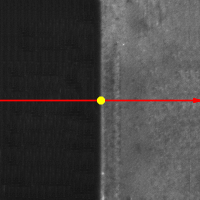
\includegraphics[width=0.275\textwidth]{img/1DEdgeDetection/edge}
& 
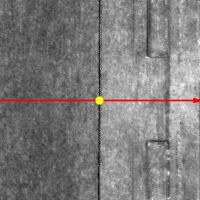
\includegraphics[width=0.275\textwidth]{img/1DEdgeDetection/ridge}
&
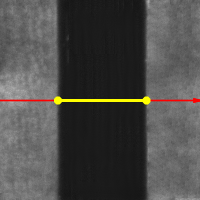
\includegraphics[width=0.275\textwidth]{img/1DEdgeDetection/stripe}
\\
\textbf{Step Edge} &
\textbf{Ridge} &
\textbf{Stripe} 
\end{tabular}
\caption{Different kinds of image features extracted from 1D profile.}
\label{tab:1DFeatures}
\end{table}
\section{Profile Extraction}

\paragraph*{}
Before we apply any of the \textbf{1D Edge Detection} methods, firstly we need to acquire a 1D profile that is to be inspected. Computing a discrete profile of image brightness along a given path is relatively straightforward task.

\paragraph*{}
The first step is to sample the scan path, selecting a set of equidistant (typically with distance of one pixel \cite[p. 150]{MVTec08}) points of interest along the path. Each of these points will correspond to one element of the constructed profile. The second step is to compute the brightness values \textit{related to} each of the points.

\subsection{Multiple Sampling}
\paragraph*{}
We used the expression \textit{related to} rather than \textit{at} on purpose - although we could simply take the image brightness values at each point of interest, it is more prudent to use an average of a series of sampling points perpendicular to the scan line, as demonsted in \reffig{MultipleSampling}; thus achieving a simple mean of noise suppression. But what kind of average should we use to compute the result for a single point of interest?

\oneFigure
{img/1DEdgeDetection/multiple_sampling_refined}
{Multiple Sampling for 1D Edge Detection.}
{MultipleSampling}
{\basicWidth}

\paragraph*{}
As long as the whole range of sampling points fits within the object being inspected and its features are perpendicular to the scan path, the brightness information collected at each of the sampling points is equally good or bad as the information collected at the other ones. Because of that we may safely use the simplest arithmetic mean.

\paragraph*{}
We will refer to the number of points used to compute a single profile value as \textit{scan width}. The wider the scan, the stronger noise attenuation we get. However, if the 2D feature we are to inspect is not perfectly perpendicular to the scan line, the wide scan area will cause the edge in the resulting 1D profile to be stretched and thus harder to identify precisely. Increasing the scan width will also increase the computation time of the profile extraction, which depends linearly on the number of sampling points.

\paragraph*{}
\reffig{EdgesProfileExtraction} demonstrates an example brightness profile extracted from the image on the right, scanned horizontally along the red scan line.

\begin{figure}[h!]
    \begin{subfigure}[b]{\basicWidth}
		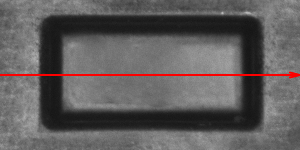
\includegraphics[width=\linewidth]{img/1DEdgeDetection/edges_scan}
    \end{subfigure}%
    ~
    \begin{subfigure}[b]{\basicWidth}
		\smallProfile{img/1DEdgeDetection/edge_profile.values}
    \end{subfigure}
    \caption{1D brightness profile extracted from the image.}
    \label{fig:EdgesProfileExtraction}
\end{figure}

\subsection{Refinement}

\paragraph*{}
Even though reasonably wide scan area suppresses the noise significantly at the extraction level, we need to keep in mind that only random noise can be suppressed in this way. Real pictures contain small features\footnote{Possibly perpendicular to the scan line and thus not affected by averaging the sampling points.} of image texture irrelevant to the inspection task that need to be attenuated before further processing of the profile. 

\paragraph*{}
Selecting the smoothing filter to refine the extracted profile is not an obvious choice. On the one hand we want to suppress the noise present in the profile, so that irrelevant intensity changes are not identified as edge points, on the other hand we want to achieve high precision of the edge localization. 

\paragraph*{}
These two criteria cannot be considered independently - smoothing of the profile suppresses the noise, but also lowers the precision. Canny determined\cite{Canny86} that the optimal trade-off between noise reduction and lose of precision is achieved with the Gaussian smoothing filter defined as follows:

\[
    g_{\sigma}(x)= \frac{1}{\sqrt{2\pi \sigma^2}} e^{-\frac{x^2}{2 \sigma^2}}
\]

where the standard deviation $\sigma$ is a parameter of the filter.

\subsubsection{Discreet Gaussian Filter}

\paragraph*{}
The Gaussian function is defined in continuous, infinite domain - to obtain a discreet approximation of the filter, we may sample $g_{\sigma}(x)$ at integer coordinates\cite{JainKasturi95}. Moreover, as the value of the Gaussian function quickly decreases with the increase of $|x|$, we may limit the discreet filter to a finite neighborhood of $x = 0$ without significant effect on the results of the smoothing. 

\paragraph*{}
The well known fact called a three-sigma rule states that more that $97\%$ of the Gaussian function integral is concentrated within $3 \sigma$ distance from $x = 0$. It is therefore reasonable to sample the Gaussian function at $2r + 1$ points, where $r$ is a small multiple of $\sigma$, e.g. $3 \lceil \sigma \rceil$; thus obtaining a mask in the following form:

\[
    \frac{1}{s} \begin{bmatrix}
    g(r) & g(r-1) & ... & g(0) & ... & g(r-1) & g(r) 
    \end{bmatrix}
\]

where $s$ equals the sum of the obtained gaussian coefficients, i.e. it ensures the mean-preservation property of the filter.

\subsubsection{Standard Deviation}

\paragraph*{}
Accurate adjustment of $\sigma$ will contribute to the robustness of the computation. We should pick a value that is high enough to eliminate noise that could introduce irrelevant extrema to the profile derivative, but low enough to preserve the actual edges we are to detect. This parameter should be adjusted through interactive experimentation on representative sample data, looking for optimal trade-off between fidelity and noise attenuation. 

\paragraph*{}
\reffig{ProfileSmoothingStdDev} demonstrates effects of smoothing the example brightness profile with different $\sigma$ values. Blue profile ($\sigma = 0.0$) exhibits fine noise while brown profile ($\sigma = 6.0$) attenuates the valleys of significant edges, which makes both suboptimal. Red profile ($\sigma = 3.0$) seems to exhibit appropriate degree of smoothing.

\profileFigure
{
	\addProfileData{img/1DEdgeDetection/edge_profile.values}
	\addProfileData{img/1DEdgeDetection/edge_profile_low_smoothing.values}
	\addProfileData{img/1DEdgeDetection/edge_profile_high_smoothing.values}
}
{Original brightness profile smoothed with different standard deviations of Gaussian operator.}
{ProfileSmoothingStdDev}


\section{Step Edges}

\paragraph*{}
Once the brightness profile is extracted and smoothed, we can proceed to detection of its features. First type that we will inspect is \textbf{step edge}. Step edges occur between two areas of different intensity and are represented as an abrupt intensity change in the 1D profile.

\subsection{Edge Operator}

\paragraph*{}
Finding the step edges in a profile requires an edge operator - an operator that produces high output for locations representing sharp change of brightness and low output for the signal plateaus. One such operator is the \textbf{derivative} of a function - an elementary concept of calculus. This is also the operator suggested by Canny in already mentioned work \cite{Canny86}. But how do we actually compute the derivative? 

\paragraph*{}
In case of a continuous signal its derivative is well defined. As both image and (consequently) its brightness profile are discreet, we are left with partial differences - discreet approximations of the signal first derivative.

\paragraph*{}
The simplest way to compute the partial difference of a discreet signal $S$ is to subtract each value from its successor, i.e.:
\[
	D[i] = S[i+1]-S[i]
\]  
This operator, called \textbf{Forward Difference}, has a slight drawback - the resulting approximation $D[i]$ actually corresponds to the domain value in between $i+1$ and $i$ (i.e to $i+\frac{1}{2}$). To achieve \textit{stable} approximation of the first derivative we can compute the value $D'[i]$ as a mean of $D[i]$ and $D[i-1]$ (\textbf{Central Difference}):
\begin{eqnarray*}
D'[i] & = & \frac{1}{2}(D[i]+D[i-1]) \\
	& = & \frac{1}{2}(S[i+1]-S[i]+S[i]-S[i-1]) \\
	& = & \frac{1}{2}(S[i+1]-S[i-1])
\end{eqnarray*}

\paragraph*{}
Both equations are feasible for our application, however we need to remember about the $\frac{1}{2}px$ shift introduced by Forward Difference operator and translate the edge points accordingly on the very end. 
\reffig{FiniteDifference} demonstrates an example finite difference profile.

\profileFigure
{
	\addProfileData{img/1DEdgeDetection/edge_profile_low_smoothing.values}
	\addProfileData{img/1DEdgeDetection/edge_profile_low_smoothing_derivative.values}
}
{An example profile and its forward difference.}
{FiniteDifference}


\subsection{Edge Points}
\paragraph*{}
Once we have computed the derivative we can identify the edge points of the original profile. There are two criteria that a profile value has to meet to be considered an edge point:
\begin{enumerate}
	\item Significant magnitude, i.e. magnitude larger than some predefined threshold.
	\item Locally maximal magnitude.
\end{enumerate}

\paragraph*{}
Both conditions are necessary - first ensures that only significant brightness changes are identified as edge points, second (called Non-Maximum Suppression) ensures that a significant but stretched edge yields only one edge point.

\paragraph*{}
The value of the minimum magnitude threshold in each case should be adjusted after inspection of derivative profile of sample data. Example depicted in \reffig{FiniteDifference} exhibits four significant peaks of the derivative profile varying in magnitude from 11 to 13, while the magnitude of its other extrema is lower than 3. In such case a value in the middle of range $(4, 10)$ would be a prudent choice of minimum magnitude threshold.

\paragraph*{}
Profile locations meeting the magnitude criteria directly translate to edge points in the original image. An example set of extracted edge points is demonstrated in \reffig{EdgesResult}.

\oneFigure
{img/1DEdgeDetection/edges_results}
{Result of \textbf{1D Edge Detection} - a list of edge points along the scan path.}
{EdgesResult}
{\basicWidth}

\subsubsection{Sub-pixel precision}

\paragraph*{}
Even though both the image being inspected and the extracted brightness profile are discreet (with pixel-precision), we can compute the local extrema of the derivative profile with sub-pixel precision thus achieving sub-pixel precision of the entire method.

\paragraph*{}
Given a local extremum of a profile $P$ at location $i$ we can fit a parabola through three consecutive profile values: $P[i-1]$, $P[i]$, $P[i+1]$ and use the x-coordinate of its peak as the location of the extremum.

\subsubsection{Edge polarity filtering}
\paragraph*{}
It is often useful to filter the extracted edge points depending on the transition they represent - that is, depending on whether the intensity changes from bright to dark, or from bright to dark.

\twoFigures
{img/1DEdgeDetection/edges_transition_bright_to_dark}
{img/1DEdgeDetection/edges_transition_dark_to_bright}
{\param{inTransition} = BrightToDark, \param{inTransition} = DarkToBright}
{EdgeTransitionPicky}
{\basicWidth}

\subsection{Post-processing}

\paragraph*{}
Once we have extracted the list of relevant edge points in the image we are nearly done. Depending on the use scenario, it may be useful to perform additional filtering of the extracted points on the very end of computation. Three methods of post-processing are particularly useful.

\subsubsection{All Edges}
\paragraph*{}
One trivial post-processing method is to simply return all of the extracted step edges, that is - not to perform any post-processing at all. That would be the default method to follow whenever we want to detect the number of edges present in the image.

\subsubsection{N Edges}
\paragraph*{}
Another option would be to select a fixed number of strongest edge points. If we know the number of edges in advance, this method allows us to disregard the adjustment of minimum magnitude threshold - we can simply set it to zero and expect that the actual edges will still be correctly located. 

\paragraph*{}
That being said, it is often useful to adjust minimum magnitude threshold anyway, so that in case of an error such as the object not being present in the image, the computation will explicitly fail instead of returning irrelevant weak edges. 

\begin{refImpl}
Step edge detection algorithms are implemented in three \studio filters. All of them share common extraction logic, differing only in post-processing method applied to select the final outcome.
\begin{itemize}
	\item \filter{ScanMultipleEdges}{1DEdgeDetection} - returns all of the extracted edgess.
	\item \filter{ScanExactlyNEdges}{1DEdgeDetection} - selects the most prominent set of edges of given cardinality.
	\item \filter{ScanSingleEdge}{1DEdgeDetection} - wrapper over previous filter which selects the single most prominent edge.
\end{itemize} 
\end{refImpl}

\section{Ridges}

\paragraph*{}
Ridges are brief bright or dark impulses on a contrasting background. Differing from step edges in their definition, they also require slightly different method of extraction. We will start the description from the point in which we have just extracted and refined the 1D profile of image brightness, as illustrated in \reffig{RidgesProfile}.

\begin{figure}[h!]
    \begin{subfigure}[b]{\basicWidth}
		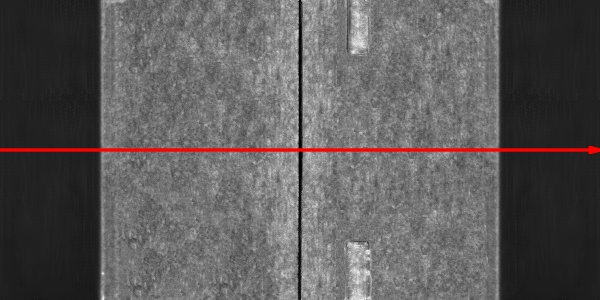
\includegraphics[width=\linewidth]{img/1DEdgeDetection/ridges_scan}
    \end{subfigure}%
    ~
    \begin{subfigure}[b]{\basicWidth}
		\smallProfile{img/1DEdgeDetection/ridges_profile.values}
    \end{subfigure}
    \caption{1D brightness profile of an image with strong ridge in its center.}
    \label{fig:RidgesProfile}
\end{figure}

\subsection{Ridge Operator}

\paragraph*{}
Ridges can be thought of as pairs of step edges of opposite polarity lying extremely close to each other. We could use this observation to propose a simple ridge detector operator adding together results of Forward Difference and Backward Difference operators:
\begin{eqnarray*}
R[i] & = & (S[i]-S[i-1])+(S[i]-S[i+1]) \\
	& = & 2S[i]-S[i-1]-S[i+1]
\end{eqnarray*}

\paragraph*{}
Such operator would be a discreet equivalent of the ridge operator proposed by Canny\cite{Canny86}, it has however two important drawbacks, pointed out by Subirana-Vilanova and Sung\cite{Subirana-VilanovaSung93}:

\begin{itemize}
	\item The operator has non-zero response for step edges, which can easily lead to false-positive errors.
	\item The quality of the detection strongly depends on the ridges having exactly 1 pixel in width, while in reality ridges usually appear as at least slightly wider.
\end{itemize}

\paragraph*{}
Both problems are illustrated by \reffig{RidgesNaiveResponse} - we can notice a high impulse response for step edges on the boundary of the object. Moreover, as the ridge in the original image has three pixels in width, it appears in the resulting profile as a pair of consecutive step edges.

\profileFigure
{
	\addProfileData{img/1DEdgeDetection/ridges_naive_operator.values}
}
{Naive ridge detection operator applied to the example profile.}
{RidgesNaiveResponse}

\paragraph*{}
The authors of \cite{Subirana-VilanovaSung93} suggest to solve the problem of high response to step edges by applying each half of the ridge operator separately and using the minimum of two responses.

\[
	R[i] = \min(S[i]-S[i-1],S[i]-S[i+1])
\]

\paragraph*{}
Such form of the operator is already feasible for narrow (one pixel wide) ridges. To successfully detect wider ridges we could define a general operator parametrized by the width of the ridge and the width of the reference margin as follows:

\begin{eqnarray*}
R[i] & = \min( & \\
	& & \overline{S[i..(i+Width)]}-\overline{S[(i-1-Margin)..(i-1)]}, \\
	& & \overline{S[i..(i+Width)]}-\overline{S[(i+1)..(i+1+Margin)])} \\
	& ) &
\end{eqnarray*}

where $\overline{S[a..b]}$ denotes the average of S values between $a$-th and $b$-th element, both inclusive.

\paragraph*{}
It should be noted that contrary to the edge detection operator which could be applied regardless of the polarity of edges being extracted, our ridge detection operator (because of the minimum function) works specifically for bright ridges. To extract dark ridges, analogous equation with maximum operator should be used.

\paragraph*{}
\reffig{RidgesProperResponse} demonstrates the outcome of using such operator on the example data from \reffig{RidgesProfile}. The maximum operator suppresses the magnitude of negative values (indicating possible ridge candidates) but amplifies the magnitude of positive values. For clarity the drawing was cropped to negative-y part.

\profileFigure
{
	\addProfileData{img/1DEdgeDetection/ridges_proper_operator.values}
}
{Amended ridge detection operator applied to the example profile.}
{RidgesProperResponse}

\paragraph*{}
Example results of ridge detection performed using such operator are demonstrated in \reffig{RidgesResults}.

\oneFigure
{img/1DEdgeDetection/ridges_result}
{Results of ridge detection.}
{RidgesResults}
{\basicWidth}

\subsection{Post-processing}

\paragraph*{}
All methods of post-processing of the extracted step edge points described in Step Edges section are applicable to ridges. 

\begin{refImpl}
Ridge detection algorithms are implemented in three \studio filters. All of them share common extraction logic, differing only in post-processing method applied to select the final outcome.
\begin{itemize}
	\item \filter{ScanMultipleRidges}{1DEdgeDetection} - returns all of the extracted ridges.
	\item \filter{ScanExactlyNRidges}{1DEdgeDetection} - selects the most prominent set of ridges of given cardinality.
	\item \filter{ScanSingleRidge}{1DEdgeDetection} - wrapper over previous filter which selects the single most prominent ridge.
\end{itemize} 
\end{refImpl}

\section{Stripes}

\paragraph*{}
Stripes are flat sections of brightness profile bounded by two step edges of opposite polarity. Such definition indicates that the problem of stripe detection heavily depends on the already discussed detection of step edges. 

\paragraph*{}
The concept of stripe is important mostly as a clear and succint means of formulation for a range of visual inspection tasks, wheareas it does not bring any novelties to the signal-processing aspect of the computation. Indeed, algorithms for stripe extraction firstly find the step edges in the profile (using previously described methods) and then process the results combining the extracted edges into stripes. 

\paragraph*{}
Next section summarizes two basic methods of combining the extracted step edges into stripes.

\subsection{Edge Processing}

\subsubsection{All Stripes}

\paragraph*{} As long as our goal is to maximize the number of constructed stripes, the problem can be solved quite efficiently. It can be easily proven that a simple $O(n)$ algorithm that greedily connects each closing edge with the first opening edge between already constructed stripes and the closing edge itself yields optimal results.

\subsubsection{N Stripes}

\paragraph*{}
The task is slightly more complicated if we know the desired number of stripes in advance and aim at maximizing the sum of strengths of step edges constituing the selected stripes. To solve such optimization problem in $O(n^2)$ time we can use a dynamic programming solution.

\paragraph*{}
Let us define a partial solution to the problem as follows:
\begin{description}
	\item \texttt{Best[Prefix][Count]} - sublist of the first \texttt{Prefix} step edges of alternating edge-polarities having \texttt{Count} elements that yields the biggest sum of edge strengths.
\end{description}

\paragraph*{}
Having computed the results for \texttt{Prefix} $=p$ we can compute the results for \texttt{Prefix} $=p+1$ in linear time - for each \texttt{Count} $=c$ we need to consider only two cases, either using the $p+1$-th step edge to extend the optimal result of \texttt{Best[p][count-1]} or not, in which case the result for the subproblem will be equal to \texttt{Best[p][count]}.

\begin{refImpl}
Stripe detection algorithms are implemented in three \studio filters. All of them share common extraction logic, differing only in post-processing method applied to select the final outcome.
\begin{itemize}
	\item \filter{ScanMultipleStripes}{1DEdgeDetection} - maximizes the number of returned stripes.
	\item \filter{ScanExactlyNStripes}{1DEdgeDetection} - constructs the most prominent set of stripes of given cardinality.
	\item \filter{ScanSingleStripe}{1DEdgeDetection} - wrapper over previous filter which selects the single most prominent stripe.
\end{itemize} 
\end{refImpl}
\section{Examples}

\paragraph*{}
In this section we will demonstrate a few industrial applications of 1D Edge Detection methods.

\subsection{Positioning}

\paragraph*{}
\textbf{1D Edge Detection} methods are commonly employed to determine locations of objects. Let us consider an image of a capsule on a production line demonstrated in \reffig{OneDEdgeDetectionPositioning}. We assume that the capsule is aligned with the axis of the image and we want to determine the range of x-coordinates occupied by the object.

\twoFigures
{img/1DEdgeDetection/positioning_edge_points}
{img/1DEdgeDetection/positioning_result}
{1D Edge Detection applied to determine capsule position along the x axis.}
{OneDEdgeDetectionPositioning}
{\basicWidth}

\paragraph*{}
As long as the background is plain and contrasting with object border, such problem can be solved easily regardless of the inner content of the object. \reffig{OneDEdgeDetectionPositioning} demonstrates the edge points detected along the horizontal scan line and visualisation of the resulting capsule position. The algorithm detects redundant, inner edges, but this does not pose a difficulty, as we only need the first and the last edge point of the returned list.

\subsection{Code Reading}

\paragraph*{}
One of the classic applications of stripe detection is reading of 1D data codes. Depending on the barcode format, we may\footnote{E.g. in case of codes from EAN/UPC family commonly used in trade.} or may not\footnote{E.g. in case of Pharmacode or Code128 standard.} know the number of bars the code is composed of - in the first case we may improve the robustness of the method using the post-processing routine for extracting the fixed number of strongest stripes which we have discussed before. In either case we expect the method to measure the width of the bars present in the image.

\oneFigure
{img/1DEdgeDetection/bars_res}
{1D Edge Detection applied to read the widths of 1D code bars.}
{OneDEdgeDetectionCodeReading}
{\basicWidth}

\paragraph*{}
It is interesting to note that the intercept theorem guarantees that we may scan the barcode at any orientation of the scan line, as long as its deviation from the barcode axis does not disrupt the stripe detection routine - the proportions of widths of the intersected bars are preserved under any orientation of the scan line.

\paragraph*{}
Once the widths of the bars are obtained they can be passed to a decoder for the specific barcode format to obtain the final reading.


%\subsection{Counting}

%\paragraph*{}
%Another popular application of \textbf{1D Edge Detection} is counting of the objects positioned along a path. Let us assume that we want to count the blades of a circular presented in \reffig{Blade}.

%\singleFigure
%{img/1DEdgeDetection/blade}
%{A circular saw blade to be inspected.}
%{Blade}
%{0.65}

%\paragraph*{}
%Such task may be solved by running a single edge detection scan along a circular path intersecting the blades. To produce the scan path we can use a straightforward \filter{CreateCirclePath}{PathBasics} filter. The built-in plugin will allow us to point \& click the required \param{inCircle} parameter, as demonstrated in \reffig{BladePlugin}.

%\singleFigure
%{img/1DEdgeDetection/blade_plugin}
%{Interactive selection of the circle parameter.}
%{BladePlugin}
%{0.5}

%\paragraph*{}
%The next step will be to pick the specific algorithm for the actual edge detection. As the objects being inspected appear as stripes in one-dimensional brightness profile and we do not know how many of them there are, the \filter{ScanMultipleStripes}{1DEdgeDetection} would be a right tool for the job.

%\paragraph*{}
%The program depicted in (...) solves the problem as expected (perhaps after increasing the inSmoothingStdDev from default of 0.6 to bigger value of 1.0 or 2.0) and detects all 30 blades of the saw.

%\twinFigure
%{img/1DEdgeDetection/blade_scan_area}
%{img/1DEdgeDetection/blade_results}
%{Scan area and the extracted stripes.}
%{BladeResults}
%{0.5}

 
\chapter{2D Edge Detection} 
\label{chap:2DEdgeDetection}

\epigraph{So no, I don't think we've lost our edge at all.}
{\textsc{Vince McMahon}}

\pagebreak

\section{Introduction}

\paragraph*{}
In the \refchap{1DEdgeDetection} chapter we have discussed a set of techniques designed to detect high-contrast features in one-dimensional profiles. Let us recall that doing so we were not interested in one-dimensional image profiles by themselves, but in two-dimensional image features intersecting the line from which the profile was extracted: we have been transferring the extracted edge points back to the original image, acquiring fragments of information about the edges present in the image.

\paragraph*{}
As we know how to detect individual edge points in an image, we may wonder if we could use the same techniques to detect entire edges - repeatedly detecting edge points and connecting them to form two-dimensional objects. The answer to this question depends on the context of the detection.

\paragraph*{}
We cannot do that when we have no information about the edges that we are going to detect, as \textbf{1D Edge Detection} techniques relay on the position and orientation of the scan line, which has to be roughly perpendicular to the primitive being inspected. However, when we do have an estimate of the feature being extracted, such approach is valid and promising - we will discuss this idea further in the \refchap{ShapeFitting} chapter.

\paragraph*{}
In this chapter we will look into the problem of \textbf{2D Edge Detection} from the ground up, incorporating the two-dimensional nature of the features into the detection algorithm, and obtain techniques that identify the edges in an image without any prior knowledge about them.

%\paragraph*{}
%Out of three primitives that we defined for one-dimensional profiles (step edges, ridges and stripes) we will discuss only edges and ridges, demonstrated in (..), as processing of two-dimensional step edges to obtain stripes is too ambiguous and complicated to be worth considering.
\section{Image Gradient}

\paragraph*{}
A derivative of a signal is a measure of local change in the signal value, and as such is a natural starting point for detection of step edges, regardless of the dimension of the space in which the signal is defined. A derivative of two-dimensional signal is usually called a \textbf{gradient}. 

In the \refchap{1DEdgeDetection} chapter we have been using partial difference operators precessed by smoothing of the signal to obtain the derivative of a profile and identify its prominent extrema as the edge points. We will translate this approach to two-dimensional space preserving its core idea - calculation of signal derivative using smoothing and partial difference operators.

\subsection{2D Partial Difference}

\paragraph*{}
To calculate the gradient of an image we may apply one of the partial difference operators discussed in the \refchap{1DEdgeDetection} chapter separately in X and Y dimension. \reffig{CentralDifferenceMasks} demonstrates appropriate convolution masks for the central difference operator.

\begin{figure}[h!]
\begin{equation*}
D_{H} = 
	\begin{bmatrix}
	-1 & 0 & 1 \\
	\end{bmatrix}\qquad
D_{V} = 
	\begin{bmatrix}
	-1 \\
	0 \\
	1
	\end{bmatrix}
\end{equation*}
\caption{Horizontal and vertical central difference masks.}
\label{fig:CentralDifferenceMasks}
\end{figure}

\paragraph*{}
In effect we obtain two images (or one two-channel image), representing vertical and horizontal derivatives at each pixel. Combining these two components into vectors representing two-dimensional gradient yields a result demonstrated in \reffig{GradientVectors}, where the resulting gradient vectors were drawn onto the original image.

\oneFigure
{img/2DEdgeDetection/GradientVectors}
{Two-dimensional image derivative computed at each pixel.}
{GradientVectors}
{\basicWidth}

\paragraph*{}
For our needs of edge detection, we are interested mainly in the magnitude of gradient vectors. \reffig{GradientMagnitude} demonstrates a gradient magnitude image, each pixel of which represents the magnitude of the corresponding gradient vector (computed using central difference operators as described above).

\twoFigures
{img/2DEdgeDetection/tooth}
{img/2DEdgeDetection/tooth_pd_amplitude}
{Gradient magnitude image of the example image.}
{GradientMagnitude}
{\basicWidth}

\paragraph*{}
We may notice that image edges are indeed discernible in such image, even though there is also significant amount of high-gradient pixels corresponding to fine features of the saw texture, rather than object edges. Sensitivity to noise was the reason for which we have incorporated Gaussian smoothing operator into our one-dimensional edge detection routines; it is clear that we need similar precautions in two dimensions.

\subsubsection{The need for simple operators}

\paragraph*{}
Even though the Canny's result\cite{Canny86} about the optimality of the derivative of Gaussian operator for edge detection applications holds for 2D, we will commence out description with simpler gradient operators, moving to Canny's method in the next section.

\paragraph*{}
Contrary to the case of one dimension, in two dimensions the amount of data to be processed is usually quite large, which creates a trade-off between accuracy and speed for real-time high-demand inspection systems. It is therefore reasonable to look into simple and fast operators, even if they are less accurate that the one advocated by Canny.

\subsection{Prewitt Operator}

\paragraph*{}
One of the first gradient operators, Prewitt operator, addresses this issue by means similar to the Multiple Sampling technique which we employed to suppress noise in profiles of image brightness at the extraction level. 

\paragraph*{}
Here the central difference operator is applied to three rows/columns in the immediate neighborhood of each pixel, which is equivalent to convolving the central difference operator witch mean average operator running in the opposite direction, as demonstrated in \reffig{PrewittMasks}.

\begin{figure}[h!]
\begin{align*}
P_{H} &= \begin{bmatrix}
	-1 & 0 & 1 
	\end{bmatrix}
	*
	\begin{bmatrix}
	1 \\
	1 \\
	1
	\end{bmatrix}
	= 
	\begin{bmatrix}
	-1 & 0 & 1 \\
	-1 & 0 & 1 \\
	-1 & 0 & 1
	\end{bmatrix} \\
P_{V} &= 
	\begin{bmatrix}
	-1 \\
	0 \\
	1 
	\end{bmatrix}
	*
	\begin{bmatrix}
	1 & 1 & 1
	\end{bmatrix}
	= 
	\begin{bmatrix}
	-1 & -1 & -1 \\
	0 & 0 & 0 \\
	1 & 1 & 1
	\end{bmatrix}
\end{align*}
\caption{Masks of the Prewitt gradient operator.}
\label{fig:PrewittMasks}
\end{figure}

\subsection{Sobel Operator}

\paragraph*{}
The quality of noise-suppression of the Prewitt operator may be improved if we replace the indiscriminate mean average with simple approximation of Gaussian smoothing, which puts emphasis on pixels nearer to the pixel at which the average is computed. Such operator was proposed by Sobel.

\begin{figure}[h!]
\begin{equation*}
S_{H} = 
	\begin{bmatrix}
	-1 & 0 & 1 \\
	-2 & 0 & 2 \\
	-1 & 0 & 1
	\end{bmatrix}\qquad
S_{V} = 
	\begin{bmatrix}
	-1 & -2 & -1 \\
	0 & 0 & 0 \\
	1 & 2 & 1
	\end{bmatrix}
\end{equation*}
\caption{Masks of the Sobel gradient operator.}
\label{fig:SobelMasks}
\end{figure}

\paragraph*{}
Nixon and Aguado provide\cite{NixonAguado08} an interesting description of derivation of similar masks for higher dimensions, where both smoothing and differencing components are obtained from Pascal's triangle, however such masks are rarely used in practice. Sobel masks of bigger dimensions approximate the Gaussian smoothing while not making use of the separability of the Gaussian kernel, which make them inferior to the actual Gaussian smoothing, as performed by Canny edge detection method.

\paragraph*{}
\reffig{SobelVsBare} compares the results of bare central difference operator with those obtained using the Sobel operator. The achieved noise suppression is not spectacular, but still noticeable.


\twoFigures
{img/2DEdgeDetection/tooth_pd_amplitude}
{img/2DEdgeDetection/tooth_sobel_aplitude}
{Comparison of bare central difference gradient (on the left) and Sobel operator gradient.}
{SobelVsBare}
{\basicWidth}


\subsubsection{Scaling}

\paragraph*{}
When we derived the masks of Prewitt and Sobel operators we neglected the scaling of the smoothing operators, i.e. we used smoothing masks such as $[1 \, 1 \, 1]$, rather than $\frac{1}{3} [1 \, 1 \, 1]$. The operators were defined in this way to allow for faster computation and are commonly used in this form.

\paragraph*{}
Whenever the smoothing operators are to be compared (or used interchangeably, e.g. in edge detection with fixed gradient magnitude threshold) it is important to remember to normalize their results, multiplying the outcome by the scaling factor of the smoothing operator omitted in the first place ($\frac{1}{3}$ for the Prewitt operator and $\frac{1}{4}$ for Sobel). Such scaling was applied to the results of the Sobel operator in \reffig{SobelVsBare}.

\begin{refImpl}
Gradient operators discussed in this section are implemented by \studio filters \filter{GradientImage\_Mask}{ImageLocalTransform} and \filter{GradientImage}{ImageLocalTransforms}.
\end{refImpl}
\section{Canny Edge Detector}

\paragraph*{}
Having discussed the concept of image gradient and a set of simple fixed-mask gradient operators, now we move our attention to the complete step edge detection technique described\cite{Canny86} by Canny (the one-dimensional version of which was our method of choice for detection of step edges in image profiles). 

\paragraph*{}
Let us recall that Canny's method for one dimension may be summarized as follows:
\begin{enumerate}
	\item Compute the derivative of Gaussian of the signal.
	\item Select the resulting points that:
	\begin{enumerate}
		\item Have magnitude above certain minimum value (\textbf{Thresholding})
		\item Have locally maximum magnitude (\textbf{Non-maximum Suppression})
	\end{enumerate}
\end{enumerate}

\paragraph*{}
Canny's method for two-dimensional edges retains this schema, but some of 2D-specific details of the individual steps are interesting enough to call for a detailed discussion.

\subsection{Gradient by derivative of Gaussian}

\paragraph*{}
The Gaussian function, which we have discussed in the \refchap{1DEdgeDetection} chapter, has a natural formulation in two dimensions:
\[
    g(x,y)= \frac{1}{2\pi \sigma^2} e^{-\frac{x^2+y^2}{2 \sigma^2}}
\]

\paragraph*{}
Apart from the optimal\footnote{Under the criteria assumed by Canny.} trade-off between noise attenuation and edge preservation, the two-dimensional Gaussian filter has two useful, 2D-specific features. The first one is \textbf{isotropy} - the response of the filter depends only on the distance from $(x,y)$ to $(0,0)$; thus the smoothing does not introduce any bias dependent on the direction of the image edges. 

\paragraph*{}
The second interesting feature is \textbf{separability}, which means that the application of the two-dimensional Gaussian filter is equivalent to successive application of two one-dimensional operators, each processing the signal in different dimension. Indeed:

\begin{align*}
    g_{\sigma}(x,y) &= \frac{1}{2\pi \sigma^2} e^{-\frac{x^2+y^2}{2 \sigma^2}} \\
    				&= \frac{1}{\sqrt{2\pi \sigma^2}} e^{-\frac{x^2}{2 \sigma^2}} \cdot \frac{1}{\sqrt{2\pi \sigma^2}} e^{-\frac{y^2}{2 \sigma^2}} \\
    				&= g_{\sigma}(x)\cdot g_{\sigma}(y)
\end{align*}

\paragraph*{}
Therefore to perform the Gaussian smoothing on an image, we may simply apply the already discussed one-dimensional smoothing operator successively to each row, and then to each column of the image. Gradient extraction based on such smoothing is demonstrated in \reffig{CannyGradient}.

\twoFigures
{img/2DEdgeDetection/tooth_canny_low}
{img/2DEdgeDetection/tooth_canny_high}
{Gradient extraction using Gaussian smoothing with different values of standard deviation ($0.7$ on the left, $2.75$ on the right).}
{CannyGradient}
{\basicWidth}

\paragraph*{}
The example results look promising - in the image on the right the outline of the object is prominent and consistently brighter that any other element of the image; the noise is effectively suppressed. On the other hand, the edges in the image clearly have excessive width, which inhibits the precision of edge localization. Conversely, image on the left exhibits fine edges, but also worse separation of edge and noise intensities. It is worth stressing that accurate adjustment of $\sigma$ is crucial for performance of the algorithm.

\subsection{Hysteresis Thresholding}

\paragraph*{}
Once we have computed the image gradient, we need to threshold the gradient magnitude image selecting the high-gradient, prospective edge locations. Although simple global thresholding described in the \refchap{ImageThresholding} chapter could be employed for that, Canny pointed out an important drawback of this method in the context of edge detection.

\paragraph*{}
Let us assume that we set the minimum magnitude threshold value to $s$, and the image contains an edge mean magnitude of which is near to $s$. Even if the illumination of the scene is uniform, the gradient magnitude of the edge pixels is bound to fluctuate around $s$ due to inevitable noise introduced by camera imperfections.

\paragraph*{}
In practice the fluctuation of edge gradient magnitude tend to be quite significant, leading to extraction of fragmented, incomplete edges. \reffig{CannyGlobalThresholding} demonstrates two ineffective global thresholding attempts on example gradient amplitude image. The results on the left are free from noise but incomplete, while lower threshold used to produce the outcome on the right introduces significant amount of noise.

\twoFigures
{img/2DEdgeDetection/tooth_canny_hist_high}
{img/2DEdgeDetection/tooth_canny_low_hist_low}
{Global thresholding of the gradient magnitude image.}
{CannyGlobalThresholding}
{\basicWidth}

\paragraph*{}
Canny proposed\footnote{This approach is a two-dimensional equivalent of the method proposed\cite{Schmitt38} by Schmitt in the context of electronic trigger, although Canny did not indicate his inspirations on that matter.} to address this issue by setting two thresholds, let us denote them by $l$ and $h$, where $l < h$. The locations of magnitude lower than $l$ are immediately discarded, while locations of magnitude higher than $h$ are immediately accepted. The locations of magnitude between $l$ and $h$ are split into connected components and each component is accepted only if it is adjacent to previously accepted (i.e. of magnitude higher than $h$) locations.

\paragraph*{}
Such topological extension of the usual thresholding, called hysteresis thresholding, proves extremely useful in edge detection applications. \reffig{CannyHysteresisThresholding} demonstrates hysteresis thresholding of the example image using two threshold values used to produce results in \reffig{CannyGlobalThresholding} as $l$ and $h$. As we can see, the edges from the low threshold image are retained in their entirety, while all of the noise is attenuated.

\oneFigure
{img/2DEdgeDetection/tooth_canny_hist}
{Hysteresis thresholding of the gradient magnitude image.}
{CannyHysteresisThresholding}
{\basicWidth}

\subsection{Non-maximum Suppression and Subpixel Precision}

\paragraph*{}
A direct translation of one-dimensional condition of locally maximal magnitude of edge locations would be to compare each pixel with its neighbors (either 4 or 8), but such approach would effectively yield only isolated, single edge locations and this is clearly not what we want.

\paragraph*{}
To derive correct translation of non-maximum suppression into two dimensions we need to remember that in 1D edge detection we were analyzing profiles perpendicular to actual image edges. As the direction perpendicular to an edge is directly represented by gradient direction, non-maximum suppression in two dimensions should be performed by comparing each pixel magnitude with its two neighbors indicated by the pixel gradient direction.

\paragraph*{}
We may use a similar approach to translate out parabola-fitting technique of acquiring sub-pixel precise positions of edge points to two-dimensions. If we sample the image at three points on the line parallel to gradient direction at a pixel and fit a parabola through the resulting, three-element profile, we obtain a direct equivalent of the fit that we were doing in one-dimensional case.

\begin{refImpl}
Edge detection method is implemented by four \studio filters, which share common logic, differing only in output data type. One can choose between Canny, Deriche and Lanser filters, or between Sobel and Prewitt algorithms when using \textit{\_Mask} version of filters.
\begin{itemize}
	 \item \filter{DetectEdges\_AsPaths}{2DEdgeDetection} - returns extracted edges as array of paths.
	 \item \filter{DetectEdges\_AsRegion}{2DEdgeDetection} - extracts edges and returns them as one region.
	 \item \filter{DetectEdges\_AsPaths\_Mask}{2DEdgeDetection} - works as DetectEdges\_AsPaths, but can be used with Sobel or Prewitt filters for gradient computing.
	 \item \filter{DetectEdges\_AsRegion\_Mask}{2DEdgeDetection} - the same as previous filter, but result is stored in region rather than in array of paths.
\end{itemize}
\end{refImpl}
%\section{Ridges}
\newcommand{\smallPath}[1]
{%
\begin{tikzpicture}
\begin{axis}[
	xtick=\empty,
	ytick=\empty,
	scale only axis,
	width=\linewidth,
	height=0.5\linewidth,
]
\addplot table[x=X,y=Y] {#1};
\end{axis}
\end{tikzpicture}
}


\chapter{Contour Analysis}
\label{chap:ContourAnalysis}

\epigraph{Be precise. A lack of precision is dangerous when the margin of error is small.}
{\textsc{Donald Rumsfeld}}

\pagebreak

\section{Introduction}

\paragraph*{}
Contour analysis can be thought of as a sub-pixel precise counterpart of \refchap{BlobAnalysis}, built upon processing of precise points organized in paths; in the same way that \refchap{BlobAnalysis} is based on processing of pixel-precise regions.

\paragraph*{}
Solutions based on contour analysis typically follow the schema of \refchap{BlobAnalysis} solutions:

\begin{enumerate}
	\item \textbf{Extraction} - sub-pixel precise paths are extracted from the image, usually by means of \refchap{2DEdgeDetection}.
	\item \textbf{Processing} - the paths are subject to transformations with an intention of rectifying the path imperfections or extracting its segments that we are particularily interested in.
	\item \textbf{Feature Extraction} - in the final part the numerical and geometrical features may be computed.
\end{enumerate}
\section{Path}

\paragraph*{}
\textbf{Path}, the fundamental data type of contour analysis, is a simple list of points defining two-dimensional curve consisting of straight segments; along with one additional, boolean information indicating if the list is \textbf{closed} or \textbf{open}, i.e., if the first point should be interpreted as connected with the last one.

\paragraph*{}
Both types of paths occur naturally as the results of \refchap{2DEdgeDetection}, as demonstrated in \reffig{PathTypes}. Paths may be also extracted from regions by computing region contours (always closed paths) or medial axis (both open and closed).

\twoFigures
{ContourAnalysis/img/ClosedPaths}
{ContourAnalysis/img/OpenPaths}
{Closed and open paths extracted in \refchap{2DEdgeDetection}.}
{PathTypes}
{\basicWidth}

\subsection{Characteristic Points}

\paragraph*{}
Each non-degenerate path represents infinite number of points on the segments between its defining points. To avoid confusion we will consequently refer to the defining points of a path as its \textbf{characteristic points}.

\subsection{Polygons}

\paragraph*{}
Let us note that our definition of path is quite general - we allow the path to have duplicate points and self-intersections. This is reasonable because a lot of important path operators (e.g. the segmentation routines which we are going to discuss soon) and features (e.g. path length) are well-defined for such paths and require no additional restrictions.

\paragraph*{}
One exception is extraction of features defined in the context of two-dimensional shapes enclosed by a path, i.e. sub-pixel precise polygons. Such operators make sense only when the path divides the space into exactly two parts - interior and exterior, and thus has to be \textbf{closed} and \textbf{not self-intersecting}.
\section{Segmentation}

\paragraph*{}
It is often the case that we are interested in a specific section of the obtained object contour, e.g. if we want to measure the angle between two specific straight segments of the object boundary. Segmentation techniques extract the sections of a path that represent simple geometric primitives such as straight segments or circular arcs.

\paragraph*{}
The task of path segmentation may be also formulated in terms of path approximation - if we approximate a path with a simple polygon, we can split it into sections corresponding to individual segments of the resulting polygon, thus obtaining segmentation into straight segments.

\paragraph*{}
The algorithm that will be our basis for developing the path segmentation methods was introduced as an algorithm for path polygonal approximation.

\subsection{Ramer Algorithm}

\paragraph*{}
Ramer proposed\cite{Ramer72} a simple and effective algorithm for approximating a path with a polygon within a given precision. The algorithm is parametrized with a value $d$, denoting maximal distance from the original curve to the resulting polygon.

\paragraph*{}
Ramer algorithm constructs the approximating polygon from the points of the original path, i.e. vertices of the resulting polygon are a subset of the original path points. The algorithm commences by approximating the whole path with a single segment: for open paths it is the segment between the path endpoints, for closed paths we may select the endpoints $a$ and $b$ of a path diameter and process two open sections of the path ($a$ to $b$, $b$ to $a$) separately.

\paragraph*{}
The algorithm proceeds recursively. At each recursive call the algorithm considers a section of the original path already approximated with a single segment $S$ and finds the point $P$ of the path section that is most distant to $S$. If the distance between $P$ and $S$ is smaller or equal to $d$, then the recursive call returns $S$ as a feasible approximation for the path section. Otherwise the path is split at $P$ and the algorithm is run recursively at each of two created sections.

\paragraph*{}
\reffig{RamerOnTooth} demonstrates the partial results of Ramer algorithm at four levels of recursion, the last image demonstrating the final outcome.

\fourFigures
{ContourAnalysis/img/ramer_tooth_after_0}
{ContourAnalysis/img/ramer_tooth_after_1}
{ContourAnalysis/img/ramer_tooth_after_2}
{ContourAnalysis/img/ramer_tooth_after_3}
{Ramer algorithm run on example path with $d = 1px$.}
{RamerOnTooth}
{\basicWidth}

\paragraph*{}
Ramer algorithm may be also used as a means of lossy compression, although such application is rarely seen in practice, as the object contours are usually quite space-efficient, at least when compared to the size of the original images.

\subsection{Straight Segments}

\paragraph*{}
Ramer algorithm may be directly applied to segment a path into straight sections. Once we have obtained the polygonal approximation, we need to split the path at the vertices of the polygon to produce an array of path sections, each of which will correspond to a segment that approximates it with the precision we have decided on.

\paragraph*{}
Results of this approach are demonstrated in \reffig{SegmentationBasedOnRamer}.

\twoFigures
{ContourAnalysis/img/ramer_tooth_after_3}
{ContourAnalysis/img/ramer_tooth_segmentation}
{Segmentation of example path into straight segments based on the output of Ramer algorithm.}
{SegmentationBasedOnRamer}
{\basicWidth}

\subsection{Circular Arcs}

\paragraph*{}
Another common type of feature that may be identified in object contours are circular arcs. A number of approach may be used to look for arciform sections directly - one idea would be to analyze turn angles at consecutive characteristic points looking for runs of roughly constant curvature, as would be expected of a circular arc. Unfortunately, this approach does not perform well for big arcs - it is often the case that the turn angles at individual characteristic points are very weak and are easily affected by noise.

\paragraph*{}
Another approach would be to adapt the Ramer algorithm to use arcs rather than straight segments. The modification is not straightforward, as two endpoints of a path section do not define a unique arc (as they did in case of segments), so we would need to fit an arc to each section by means of \refchap{ShapeFitting}. While this does not pose a big problem, we may note that the contours being inspected rarely consist solely of circular arcs\footnote{Full circles are a common case, but these represent a single primitive and thus do not need to be segmented.}; usually they are a combination of of straight and arciform sections.

\paragraph*{}
To obtain a technique that would segment a path into sections of both types, we may start with the classic Ramer-based segmentation into straight sections and post-process its results, joining together short parts that would be well approximated by an arc.

\paragraph*{}
One approach for such post-processing would be to fit an arc to each pair of consecutive sections of Ramer-segmented path and compute the maximum distance between the path and the arc, as well as the path and its current approximation\footnote{Two straight segments or an arc in case of a part that is a result of such joining itself.}. If the maximum distance to the arc is lower, we may conclude that the arc is better approximation for the consecutive segments and join these together. This routine would be continued until convergence and in the end we would classify the sections that resulted in such joining as arciform and the others as straight.

\paragraph*{}
Two problems may be encountered when this method is applied:

\begin{itemize}
	\item When the arc being fit to a pair of consecutive straight sections has especially big radius and small length, so that it is close to a segment, the resulting improvement of the approximation is tiny and classification of the part as an arciform section may be confusing.
	\item Once two straight sections are joined, the resulting arc approximation may be so accurate that it will preclude further joining of the resulting section - a perfectly arciform path initially segmented into numerous straight parts has little chances of being fully joined.
\end{itemize}

\paragraph*{}
First issue may be addressed by limiting the radii of the arcs being fitted to a predefined threshold (which will be a parameter of the algorithm) - if the resulting arc is to big we simply do not join the sections we are considering. This simple solution is perfectly feasible as long as the arcs we intend to extract have reasonably high relation of length to radius.

\paragraph*{}
A natural solution to the second problem is indiscriminate joining of the consecutive sections whenever the maximum distance between the path section and the fitted arc is within the maximum distance we used for the initial Ramer segmentation.

\paragraph*{}
\reffig{SegmentationStraightAndArciform} demonstrates an example application of Ramer segmentation with post-processing with the amendments described above.

\fourFigures
{ContourAnalysis/img/round_contour}
{ContourAnalysis/img/round_initial}
{ContourAnalysis/img/round_straight}
{ContourAnalysis/img/round_arciform}
{Initial segmentation of the example contour (a) into straight segments (b) and results of post-processing: straight (c) and arciform (d) path segments.}
{SegmentationStraightAndArciform}
{\basicWidth}

\begin{refImpl}
\studio filter \filter{ReducePath}{PathGlobalTransforms} implements the Ramer algorithm, while \filter{SegmentPath}{PathGlobalTransforms} implements the segmentation technique built upon it as described above.
\end{refImpl}
%\section{Features}

\section{Statistical Features}

\subsection{Polygon Moments}

\paragraph*{}
In the \refchap{BlobAnalysis} chapter we have discussed region moments - generalized statistical features based on region pixel coordinates. Equivalent formulas may be formulated for sub-pixel precise polygons - yet we will need to perform an integraton over the polygon surface rather than simple summation, as the number of points contained in a non-degenerate polygon is infinite.

\paragraph*{}
In the following equations we assume $S$ to be a polygon defined by a closed, not self-intersecting path. The raw and central moments of $S$ are defined as:

\begin{align*}
	m_{p,q} &= \iint_{(x,y) \in S} x^p y^q dx dy \\
	c_{p,q} &= \iint_{(x,y) \in S} (x-\overline{x})^p (y-\overline{y})^q dx dy
\end{align*}

and both may be normalized, i.e. divided by the area $a$ of $S$:

\begin{align*}
	m'_{p,q} &= \frac{1}{a} m_{p,q}\\
	c'_{p,q} &= \frac{1}{a} c_{p,q}
\end{align*}

\subsection{Computation}

\paragraph*{}
As opposed to region moments, the formulas for shape moments do not give us a direct algorithm for computing any of them - in each case we are left with a double integration to perform.

\paragraph*{}
Luckily, Green's theorem defines the relation between any double integral over simple polygon and line integral over its boundary, which allow to substitute double integral by a sum of line integrals, each of which will be evaluated over a segment of the boundary path. For the line integrals of low order, closed formulas may be obtained, as given\cite{Turkowski97} by Turkowski for first and second-order moments.

\paragraph*{}
For instance, this approach allows to obtain the following formula for zeroth moment of a shape defined by a closed, $n$-point path $S$:
\[
	m_{0,0} = \frac{1}{2} \sum_{p = 0}^{n-1} (S[p]_x \cdot S[p+1]_y  - S[p+1]_x \cdot S[p]_y)
\]
which is the well known formula for the area of polygon based on the cross product of vectors from $(0,0)$ to its consecutive vertices. 

\paragraph*{}
From the practical point of view it is important that the polygon moments can be computed precisely, deterministically in linear time (in terms of the number of their characteristic points).

\subsection{Applications}

\paragraph*{}
As the order of moments (defined as a sum of the moment exponents, i.e. $p+q$ for $m_{p,q}$) increases, the shape-describing information carried by them gets harder for interpretation and conscious use. In the field of industrial inspection usage of moments is usually focused on the moments of order $0$, $1$ and $2$.

\subsubsection{0th order}

\paragraph*{}
There is only one zeroth moment - $m_{0,0}$, which equals the \textbf{area} of the shape. Having both exponents equal to zero, this moment indeed ignores the values of both coordinates of the points contained by the polygon. Apart from direct applications, this moment is frequently evaluated to normalize (i.e. divide by the area) the other, higher-order shape moments.

\subsubsection{1st order}

\paragraph*{}
First order moments are the first moments the normalization of which yields useful information. The moments $m'_{1,0}$ and $m'_{0,1}$ represent, respectively, the average $x$ and $y$ point coordinates of the shape. Together they form the \textbf{mass center} of the shape -  if we imagine the shape as a flat, rigid body, then it would remain in balance when positioned over a point support in its mass center.

\paragraph*{}
The mass center allow us to define certain geometric features, such us the shape \textbf{radius}, which we will discuss in the next section.

\subsubsection{2nd order} 

\paragraph*{}
Second order moments are the first moments that reflect the relation between $x$ and $y$ point coordinates of the shape, and as such, are particularly interesting. Extracting practical information about a shape from its second order moments is not trivial though - to do so we will return to the mechanical analogy of flat rigid body, which we have just introduced.

\paragraph*{}
Under such interpretation, the matrix of the second order central moments of the shape:
\[
I = \begin{bmatrix}
c'_{2,0} & c'_{1,1}\\
c'_{1,1} & c'_{0,2}
\end{bmatrix}
\]
represents an important concept of mechanics - \textbf{tensor of inertia}, which determines the torque needed to rotate a shape around any axis going through its mass center (in a similar way that a mass of a body determines the force needed to give the body the desired acceleration). The torque $T$ needed to change the angular velocity of the body by $\omega$ may be calculated as follows:
\[
	T = I\omega
\]

\paragraph*{}
Although $I$ determines the inertia for rotation around any axis going through the mass center, some of them are of particular interests - the principal axes $\omega'$, which yield stable rotation, i.e. preserve the direction of angular momentum. These axes represent the eigenvectors of $I$ and as such may be obtained directly from shape moments.

\paragraph*{}
\reffig{AxesOfInertia} demonstrates the principal axes of inertia of two example shapes.

\twoFigures
{BlobAnalysis/img/moments_capsule}
{BlobAnalysis/img/moments_meter}
{Principal axes of inertia (marked in red and yellow) of example shapes (marked in orange).}
{AxesOfInertia}
{\basicWidth}

\paragraph*{}
Interestingly, these axes may be also obtained using another, yet equivalent approach: as the axes of an ellipse having the same moments up to the second order as the shape being considered. An exhaustive description may be found in the textbook\cite[p.~73-75]{Haralick92} by Haralick and Shapiro.

\paragraph*{}
The principal axes allow to define at least two useful shape features:
\begin{itemize}
	\item \textbf{Orientation} - the direction of the major principal axis.
	\item \textbf{Elongation} - the quotient of major principal axis length and minor principal axis length.
\end{itemize}  

\begin{refImpl}
The following \studio filters extract the statistical features of a polygon: 
\filter{ShapeArea}{ShapeFeatures}, 
\filter{ShapeElongation}{ShapeFeatures}, 
\filter{ShapeMassCenter}{ShapeFeatures}, 
\filter{ShapeOrientation}{ShapeFeatures},
\filter{ShapeEllipticAxes}{ShapeFeatures}. 
\end{refImpl}

\section{Geometrical Features}

\subsection{Radius and Diameter}

\paragraph*{}
The principal axes of inertia which we have discussed recently provide approximate information about the dimensions of the shape. Strict, geometrical measures may be obtained as generalizations of basic features of circles: radius and diameter.

\paragraph*{}
\textbf{Radius} of a shape may be defined as the maximum distance between its mass center and any of its points. It is not hard to prove that such point has to be a characteristic point of the polygon, and therefore may be found in a straightforward search.

\paragraph*{}
\textbf{Diameter} of a shape may be defined as the maximum distance between any two points of the shape. Also in this case in may be shown that such points are always the characteristic points of the polygon and as such may be found in $O(n^2)$ time. This result may be improved to $O(n\log n)$ using the rotating calipers technique\cite{Toussaint83} on the convex hull of the polygon (see below).

\paragraph*{}
Both these features offer an alternative definition for the \textbf{orientation} of a polygon - the vector from the mass center of the shape to the most distant point (corresponding to shape radius) is especially interesting, as it yields result in full range ($0^{\circ}$, $360^{\circ}$), as opposed to the moment-based orientation or the orientation of the diameter, which are limited to the ($0^{\circ}$, $180^{\circ}$) range.

\subsubsection{Convex Hull and Convexity}

\paragraph*{}
\textbf{Convex hull} is the smallest convex polygon that contains a set of points. Finding such polygon is a classic problem of computational geometry for which numerous efficient algorithms has been developed. Popular textbook by Cormen et al. covers\cite{Cormen01} some of them, probably the most popular one being the Graham algorithm.

\paragraph*{}
Slightly less frequently mentioned method\cite{Andrew79} by Andrew preserves the general idea of Graham algorithm yet uses lexicographic rather than angular sorting, which is simpler and less prone to errors (e.g. due to the imperfections of the floating-point representation) and as such it is worth considering for practical applications.

\paragraph*{}
Once we know how to compute the convex hull of a path we may define a convexity factor of a shape as the quotient of the area of the shape and the area of its convex hull. The obtained numeric feature allows to estimate the magnitude of cavities and holes present in the objects being inspected.

\subsubsection{Circle and Circularity}

\paragraph*{}
One trivial method to find the smallest circle containing a set of points is based on an observation, that such circle has to have some three of the given points on its boundary (or two in a special case when the points lie on the circle diameter) - otherwise we could shrink the circle and still cover all of the points. 

\paragraph*{}
We may therefore iterate over all triples of the given points, compute a unique circle passing through each of them and select the smallest feasible (i.e. covering all points) circle. Such solution would work in $\Theta(n^4)$ time, $n$ denoting the number of given points, which may result in a significant computational burden even for relatively short paths.

\paragraph*{}
Much faster solution based on iterative improvement was proposed\cite{Welzl91} by Welzl - his randomized algorithm achieves linear expected running time and allows for a concise, recursive implementation.

\paragraph*{}
We may define at least three reasonable numerical features that reflect the similarity between a given shape and a circle:
\begin{enumerate}
	\item Quotient between the area of the shape and the area of its bounding circle.
	\item Quotient between the area of the shape and the area of a circle with the same radius.
	\item Quotient between the area of the shape and the area of a circle with the same perimeter.
\end{enumerate}
All of these features assume values between $0$ and $1$, $1$ being achieved for perfect circles. The selection of particular method should be based on the nature of expected deviation of the shape from a perfect circle. For instance, the second method, being based on a radius of the shape, will be particularly responsive to \textbf{elongated} shapes, while perimeter-based feature will be sensitive to high \textbf{curvature} of the object boundary.

\begin{refImpl}
Some of the features being discussed in this section are well defined for all paths, including open and self-intersecting ones. These features are implemented in \studio by filters from the Path Features category:
\filter{PathBoundingBox}{PathFeatures},
\filter{PathBoundingCircle}{PathFeatures}, 
\filter{PathBoundingRectangle}{PathFeatures}, 
\filter{PathConvexHull}{PathFeatures},
\filter{PathDiameter}{PathFeatures} and
\filter{PathLength}{PathFeatures}.

\paragraph*{}
The following \studio filters extract the features defined only for polygons: 
\filter{ShapeConvexity}{ShapeFeatures}, 
\filter{ShapeCircularity}{ShapeFeatures} and 
\filter{ShapeRectangularity}{ShapeFeatures}.
\end{refImpl}
%\section{Examples} 
\chapter{Shape Fitting} 
\label{chap:ShapeFitting}

\epigraph{Geometry was the first exciting course I remember.}
{\textsc{Steven Chu}}

\pagebreak


\section{Introduction}

\paragraph*{}
Images being subject to interpretation in industrial inspection tasks often contain simple geometric shapes such as segments and circles. Precise extraction of such features is the key point for various measurement tasks, such as calculating the diameter of a cylinder head, demonstrated in \reffig{RadiusOfCylinderHead}.

\twoFigures
{ShapeFitting/img/head}
{ShapeFitting/img/measure_radius}
{Example application of shape fitting - the diameter of a cylinder head is calculated indirectly as the diameter of a circle fitted to the image.}
{RadiusOfCylinderHead}
{\basicWidth}


\paragraph*{}
Various approaches may be taken to obtain abstract information about the geometrical primitives represented in an image. Famous Hough transform performs an exhaustive search iterating through the space of all possible shapes, e.g. all possible radii and centers of circles, within a predefined constraints and with a predefined precision. Each candidate is verified using gradient direction information at the pixels that it is expected to intersect.

\paragraph*{}
Unfortunately, such approach often proves computationally demanding and easy to disrupt by the imperfections of the shape being identified. Moreover, the method requires careful calibration of the search space constraints and precision of the search. \reffig{HoughProblem} demonstrates a typical problem that occurs frequently when the precision of the search is too low, causing the Hough transform to yield multiple results, none of which is accurate.

\oneFigure
{ShapeFitting/img/HoughWithFixedRadius}
{Hough transform-based circle detection performed on the example image.}
{HoughProblem}
{\basicWidth}

\paragraph*{}
An alternative solution would be to apply one or two-dimensional \textbf{edge detection} to extract a group of edge points on the boundary of the shape being examined and fit the abstract shape to such points.

\paragraph*{}
In this chapter we will overview the classic methods of fitting lines and circles to sets of points in two-dimensional space. We will also demonstrate a particularily useful technique based on one-dimensional edge detection and shape fitting that allow to fit approximate positions of abstract primitives to their actual occurences.
\section{Lines}

\paragraph*{}
The problem of fitting lines to data frequently occurs in the field of statistics, where it is called \textit{linear regression}. In this context the aim of the fitting is to find a line in the form $y = ax + b$ that optimally models the relation between the (controlled, error-free) variable $x$ and (possibly affected by errors) $y$, given a set of data samples $(x_i, y_i)$. 

\paragraph*{}
The popular slope-intercept representation of lines works well for statistical regression, where the $x_i$ of data samples are unique, but causes problems in the general case, as the vertical lines can not be represented in this form and nearly-vertical lines require extremely high magnitude of the slope parameter, jeopardizing the numeric stability of the computation. We will therefore use the general equation of a line:
\[
	\{(x,y): ax + by + c = 0\}
\]
together with a normalization condition:
\[
	\sqrt{a^2 + b^2} = 1 
\]

\paragraph*{}
The normalization of the vector $(a,b)$ asserts that every line has a unique representation and inherently includes the necessary requirement of $(a,b) \neq (0,0)$. It also allows easy computation of the distance between the line and any point $(x_i,y_i)$, which equals:

\[
	\frac{|ax_i + by_i + c|}{\sqrt{a^2 + b^2}} = |ax_i + by_i + c|
\]

\subsection{Problem Formulation}

\paragraph*{}
From the above, we can formulate a concise definition of the optimization problem that we want to solve for any set of points $P$. Assuming the standard least-squares criterion that aims at minimization of the squared distances from each points to the resulting line, we wish to minimize the following function:

\[
	\sum_{(x,y) \in P} (ax + by + c)^2
\]

over all lines $(a,b,c)$ that meet the criterion $\sqrt{a^2 + b^2} = 1$.

\subsection{Moment-based Solution}

\paragraph*{}
Interestingly, it turns out that we have already discussed almost identical problem, although stated rather covertly. Minimization of the squared distances from a point set to a line is, under physical terminology, nothing else that finding the axis of minimal inertia of the point set; as its moment of inertia equals the sum of squared distanced from each point to the axis of rotation.

\paragraph*{}
As we have already indicated in the \refchap{ContourAnalysis} chapter, such axis may be computed as the eigenvalue of the inertia tensor of the rigid body:
\[
I = \begin{bmatrix}
c'_{2,0} & c'_{1,1}\\
c'_{1,1} & c'_{0,2}
\end{bmatrix}
\]

\paragraph*{}
All that we need to do to adapt this solution to our needs is to define the moments of a point set $P$, which are directly equivalent to the moments which we have defined for regions:

\begin{align*}
	m_{p,q} &= \sum_{(x,y) \in P} {x}^p {y}^q \\
	c_{p,q} &= \sum_{(x,y) \in P} ({x}-\overline{x})^p ({y}-\overline{y})^q
\end{align*}

\paragraph*{}
Equivalent result may be also obtained directly using multivariate analysis - the derivation may be found in \cite[p.~588-591]{Haralick92}.

\paragraph*{}
\reffig{LineFittingResults} demonstrates example results of least-squares line fitting.

\twoFigures
{ShapeFitting/img/line_clean_fit}
{ShapeFitting/img/line_outliers_fit}
{Example results of least-squares line fitting.}
{LineFittingResults}
{\basicWidth}

\subsection{Outlier Suppression}

\paragraph*{}
It is often the case that, due to the imperfections of edge extraction or the object being analyzed, the input data contains points that do not represent accurately the shape that we wish to extract; as demonstrated in the image on the right of \reffig{LineFittingResults}. Such points, called outliers, distort the outcome of the fitting and should be skipped or suppressed in the computation.

\subsubsection{Random Sample Consensus}

\paragraph*{}
Random Sample Consensus, proposed\cite{FischlerBolles81} by Fischler and Bolles, is a popular, probabilistic method of robust estimation that exhibits good performance against outliers, even when they represent a significant fraction of the data.

\paragraph*{}
The method iteratively selects a random minimal sample of points that allows an estimation of the results, in our case that would be a pair of points, to which a line $L$ is fitted. After each such estimation the algorithm counts the data points that \textit{support} the estimate, i.e. lie within a predefined distance $d$ from $L$. 

\paragraph*{}
The algorithm terminates after a predefined number of iterations, fitting a line to all points that supported the most supported estimate.

\paragraph*{}
The major drawback of such approach in the context of industrial applications is its probabilistic nature - for the robustness of the systems being designed it is crucial that the methods being deployed should succeed and fail deterministically and consistently on similar data instances.

\subsubsection{Iterative Suppression}

\paragraph*{}
Another, more predictable in its outcomes, approach would be to improve the results of the fitting iteratively, progressively suppressing the influence of the points that are distant from the estimates being obtained. 

\paragraph*{}
After each least-squares fit yielding a line $L$, we may calculate the distances between each data point and $L$ and inspect the distribution of distances looking for possible outliers. If we compute a nonnegative weight $w_i$ for each point reflecting our belief that the point $i$ is not an outlier, we could limit the influence of the points with low weight using weighted moments defined as follows:

\begin{align*}
	m_{p,q} &= \sum_{(x,y,w) \in P} w {x}^p {y}^q \\
	m'_{p,q} &= \frac{1}{t} m_{p,q} \\
	c_{p,q} &= \sum_{(x,y,w) \in P} w ({x}-\overline{x})^p ({y}-\overline{y})^q \\
	c'_{p,q} &= \frac{1}{t} c_{p,q}
\end{align*}

where $t = \sum_{(x,y,w) \in P} w$ is a sum of all weights. Such values would be used instead of the classic moments in the successive iteration of the algorithm.

\paragraph*{}
There are a number of possibilities regarding the specific methods of calculating the weights $w_i$ given the distances $d_i$ between each point and the last estimate of the line. A classic method proposed by Huber computes the weights as:

\[
  w_i = \left\{ 
  \begin{array}{l l}
    1 & \quad d_i \leq t\\
    \frac{t}{d_i} & \quad d_i > t\\
  \end{array} \right.
\]

where the threshold $t$ may be either calculated from the distribution of distances $d_i$ (e.g. as its median) or be left as a parameter of the algorithm. Example results of iterative outlier suppression are demonstrated in \reffig{LineFittingOutlierSuppresion}.

\twoFigures
{ShapeFitting/img/line_outliers_fit}
{ShapeFitting/img/line_outliers_fit_with_suppresion}
{Example results of line fitting without and with outlier suppression.}
{LineFittingOutlierSuppresion}
{\basicWidth}

\subsection{Segments}

\paragraph*{}
Line fitting may be directly applied to fit segments to data points, as we may start with fitting a line to the points and then compute the resulting segment as a section of the line defined by the orthogonal projection of the input points onto the line.

\begin{refImpl}
\studio filter \filter{FitLineToPoints}{GeometryFeatures} implements the line fitting along with optional iterative outlier suppression, while the \filter{FitSegmentToPoints}{GeometryFeatures} performs analogous segment fitting.
\end{refImpl}
\section{Circles}

\paragraph*{}
We now move our attention to the problem of circle fitting. A canonical equation used to represent circles is the following:

\[
	\{(x,y): (x-a)^2 + (y-b)^2 = r^2\}
\]

where $(a,b)$ is the center of the circle and $r$ denotes its radius. Under this representation, distance between the circle and a point $(x_i, y_i)$ is given by:

\[
	|\sqrt{(x_i-a)^2 + (y_i-b)^2} - r|
\]

\paragraph*{}
The least-squares circle fit to a point set $P$ may be therefore formulated as the minimization of the error:

\[
	\sum_{(x,y) \in P} (\sqrt{(x-a)^2 + (y-b)^2} - r)^2
\]

over possible circles $(a,b,r)$.


\paragraph*{}
Unfortunately, this problem is nonlinear and cannot be solved by a finite algorithm. The existing methods for circle fitting may be divided into two groups: iterative algorithms that optimize the least-squares function defined above (these methods are usually referred to as \textit{geometric}) and methods that optimize other, easier to solve, cost functions (these methods are usually called \textit{algebraic}).

\paragraph*{}
The geometric fit is theoretically enticing, but causes significant problems in practical applications. Every algorithm trying to find the least-squares fit is inherently prone to divergence or convergence to suboptimal local minimum. Moreover, the geometric fit algorithms tend to be computationally expensive, at least when compared with the popular methods of algebraic fitting.

\paragraph*{}
At the same time the best available methods of algebraic fitting yield accurate, close-to-optimal results and are free from this limitations - both experimental and theoretical arguments on this issue can be found in an exhaustive work\cite{Chernov10} of Chernov.

\subsection{Algebraic Fit}

\paragraph*{}
Perhaps the simplest method of algebraic circle fitting was given by Kasa, who proposed to minimize the following error function:

\[
	\sum_{(x,y) \in P} ((x-a)^2 + (y-b)^2 - r^2)^2
\]

\paragraph*{}
After a simple substitution $A = -2a$, $B = -2b$, $C = a^2 + b^2 - r^2$ and introducing artificial, third dimension of the point set $z = x^2 + y^2$ we get:

\[
	\sum_{(x,y) \in P} (z + Ax + By + D)^2
\]

\paragraph*{}
The minimum of this function can be found by computing the partial derivatives with respect to $A$, $B$, $C$ - we require that each such derivative is equal to zero at the minimum, which leads to the following system of linear equations:

\begin{align*}
	m'_{2,0,0}A + m'_{1,1,0}B + m'_{1,0,0}C &= -m'_{1,0,1}\\
	m'_{1,1,0}A + m'_{0,2,0}B + m'_{0,1,0}C &= -m'_{0,1,1}\\
	m'_{1,0,0}A + m'_{0,1,0}B + C &= -m'_{0,0,1}
\end{align*}

where $m'_{p,q,s}$ denotes three-dimensional (together with the artificial dimension $z$), normalized moments. Such system can be solved efficiently by methods of linear algebra.

\paragraph*{}
Kasa's method has a number of advantages: it is very fast, it is easy to implement, and its moment-based schema is easy to equip with the iterative outlier suppression which we have described in the last section. Its major weakness is poor performance on data representing small arcs (10 degrees or less), for which it often fails to yield a feasible estimation.

\paragraph*{}
Fortunately, more advanced methods of algebraic fitting by Pratt and Taubin achieve far better performance retaining the advantages of the algebraic fit. Details of these methods as well as a benchmark of their performance are given in the already mentioned work\cite{Chernov10}, which indicates the Taubin method as feasible for the majority of practical applications.  

\paragraph*{}
\reffig{AlgebraicFitResults} demonstrates the results of Kasa and Taubin fit for the data set representing small circular arc.

\twoFigures
{ShapeFitting/img/AlgebraicFit_Kasa}
{ShapeFitting/img/AlgebraicFit_Taubin}
{The algebraic fit of Kasa (on the left) and Taubin (on the right).}
{AlgebraicFitResults}
{\basicWidth}

\subsection{Circular Arcs}

\paragraph*{}
Circle fitting may be easily modified to return circular arcs rather than full circles. Again, all that we need to do is to compute the orthogonal projection of the input points onto the resulting circle and select the smallest section of the circle that contains all projection points.

\begin{refImpl}
\studio filter \filter{FitCircleToPoints}{Geometry2DFitting} implements a selection of algebraic line fitting methods along with optional iterative outlier suppression, while the \filter{FitArcToPoints}{Geometry2DFitting} performs analogous fitting of circular arcs.
\end{refImpl}
\section{Fitting Approximate Primitives to Images}

\paragraph*{}
Utilizing the shape fitting techniques in the context of image analysis requires extraction of the points to which the primitives will be fitted. Typically such extraction is done by means of \refchap{1DEdgeDetection} or \refchap{2DEdgeDetection}, which allow to fit the shapes to step edges or ridges present in the image.

\paragraph*{}
The methods of \refchap{1DEdgeDetection} allow to build particularly useful technique for fitting approximately positioned primitives to their actual occurences. The idea is to take a rough estimation of the primitive location and construct a set of scan lines going across the approximate primitive. By performing one-dimensional edge or ridge detection along each scan line, we obtain a set of points that, hopefully, represent the actual position of the primitive being located.

\paragraph*{}
In \reffig{FitSegmentToEdges} a segment is fitted to the edge of an object, while \reffig{FitCircleToRidges} demonstrates an example of fitting a circle to a circular ridge.

\twoFigures
{ShapeFitting/img/SegmentToEdges_Scans}
{ShapeFitting/img/SegmentToEdges_Result}
{Shape fitting applied to fit a segment to an edge.}
{FitSegmentToEdges}
{\basicWidth}

\twoFigures
{ShapeFitting/img/CircleToRiges_Scans}
{ShapeFitting/img/CircleToRiges_Result}
{Shape fitting applied to fit a circle to a ridge.}
{FitCircleToRidges}
{\basicWidth}

\begin{refImpl}
\studio provides filters for each type of primitive, one filter of a pair fitting the primitive to image edges, second - to image ridges, and third - to image stripes:
\begin{itemize}
	\item \filter{FitArcToEdges}{ShapeFitting}, \filter{FitArcToRidges}{ShapeFitting}, \filter{FitArcToStripe}{ShapeFitting}
	\item \filter{FitCircleToEdges}{ShapeFitting}, \filter{FitCircleToRidges}{ShapeFitting}, \filter{FitCircleToStripe}{ShapeFitting}
	\item \filter{FitPathToEdges}{ShapeFitting}, \filter{FitPathToRidges}{ShapeFitting}, \filter{FitPathToStripe}{ShapeFitting}
	\item \filter{FitSegmentToEdges}{ShapeFitting}, \filter{FitSegmentToRidges}{ShapeFitting}, \filter{FitSegmentToStripe}{ShapeFitting}
\end{itemize}
\end{refImpl}
\section{Examples}

\subsection{Measurements}

\paragraph*{}
\reffig{MeasureAngle} demonstrates an application of the shape fitting in which it is used to measure the angle between two edges of a saw tooth.

\twoFigures
{ShapeFitting/img/measure_angle_scan}
{ShapeFitting/img/measure_angle_res}
{An example application of shape fitting.}
{MeasureAngle}
{\basicWidth}

\chapter{Template Matching} 
\label{chap:TemplateMatching}

\epigraph{If Edison had a needle to find in a haystack, he would proceed at once with the diligence of the bee to examine straw after straw until he found the object of his search. 
\linebreak \linebreak
A little theory and calculation would have saved him ninety per cent of his labor.}
{\textsc{Nikola Tesla}}

\pagebreak

\section{Introduction}

\paragraph*{}
We have already discussed a number of methods that may be utilized for object localization. For instance - we can use simple \refchap{ImageThresholding} (possibly together with \refchap{BlobAnalysis}) to identify objects of contrasting brightness. \refchap{1DEdgeDetection} may be applied to locate object boundaries whenever we already know its approximate position. \refchap{ContourAnalysis} allows to identify objects by analysis of the paths which we have previously extracted using \refchap{2DEdgeDetection} etc.

\paragraph*{}
While these methods allow to construct \textbf{tailored solutions} for particular applications, identification problems may turn out to be too complex to allow for convenient application of any of the above. Moreover, specialized solutions are inherently coupled with the particular object to be found, which makes it hard to update the inspection system once the problem specification changes (e.g. because one of the components used in production is replaced by another).

\paragraph*{}
In this chapter we will discuss the most general-purpose technique of object localization - \textbf{template matching}, which allow to identify parts of an image that match, under some criterion of similarity, arbitrarily chosen image template. Such methods not only allow to solve identification problems that otherwise could not be tackled, but also provide a convenient (yet often more computationally expensive) alternative to the methods that we have discussed before. 

\twoFigures
{TemplateMatching/img/board_template_padded}
{TemplateMatching/img/board}
{An example input for a template matching problem - occurrences of the template depicted on the left are to be found in the image of the right.}
{TemplateMatchingBoardInput}
{\basicWidth}

\paragraph*{}
The crucial part of any template matching method is the specific measure of image similarity that will be used to evaluate the possible matches. We need such measure not only to design the algorithm, but also to define the task in the first place - if we are supposed to find the template occurrences, we need to specify what does it mean that a template \textit{occurs} at some position in the image. 

\paragraph*{}
A template aligned over an image at some position corresponds to a section of the image that it overlaps. If we assume that the possible template alignments are pixel-precise, the problem of evaluating the quality of the match is essentially a problem of calculating the similarity of two images of equal dimensions.

\paragraph*{}
In this chapter we will discuss two groups of template matching techniques, differing in image similarity measure they are built upon:

\begin{itemize}
	\item \textbf{Brightness-based matching} evaluates the image similarity using brightness properties of the images.
	\item \textbf{Edge-based matching} compares the gradient-based features of both images.
\end{itemize}

\section{Brightness-Based Matching}

\paragraph*{}
Brightness-based matching evaluates possible template alignments using measures of image similarity based on the relation between the brightness of the corresponding pixels of the images being compared.

\subsection{Image Correlation and Image Difference}

\paragraph*{}
While some of the measures of image similarity have natural formulation which yields high values for well-correlated images and low values for images that differ significantly, other are easier to define conversely, as measures of difference between images. To distinguish between these two groups we will use the term \textbf{image correlation} when referring to direct measures of image similarity and \textbf{image difference} when considering measures of dissimilarity. Naturally, both are equally suitable for our needs.

\paragraph*{}
We will discuss three important measures of image similarity in the context of a simple comparison benchmark demonstrated in \reftab{ImageSimilarityMeasures}.

\begin{table}[h!]
\centering
\begin{tabular}{| m{.02\linewidth} m{.13\linewidth} m{.13\linewidth} m{.12\linewidth} m{.12\linewidth} m{.12\linewidth} | }
\hline
 & & & \textbf{ME} & \textbf{MSE} & \textbf{NCC} \\
(a) & 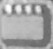
\includegraphics[width=.13\textwidth]{TemplateMatching/img/board_template} & 

\includegraphics[width=.13\textwidth]{TemplateMatching/img/board_tcomp_empty} &
54.196 & 3933.365 & 0.090 \\
(b) & 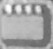
\includegraphics[width=.13\textwidth]{TemplateMatching/img/board_template} & 
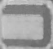
\includegraphics[width=.13\textwidth]{TemplateMatching/img/board_tcomp_detail} &
8.455 & 623.833 & 0.702 \\
(c) & 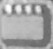
\includegraphics[width=.13\textwidth]{TemplateMatching/img/board_template} & 
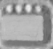
\includegraphics[width=.13\textwidth]{TemplateMatching/img/board_tcomp_another} &
10.894 & 271.555 & 0.866 \\
(d) & 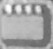
\includegraphics[width=.13\textwidth]{TemplateMatching/img/board_template} & 
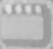
\includegraphics[width=.13\textwidth]{TemplateMatching/img/board_tcomp_linear} &
18.528 & 550.718 & 1.000 \\ \hline
\end{tabular}
\caption{Image similarity measures evaluated on example image pairs.}
\label{tab:ImageSimilarityMeasures}
\end{table}

\subsubsection{Mean Error (ME)}

\paragraph*{}
Perhaps the simplest measure of image difference is the average of its pixel-wise differences, i.e.:
\[
	\mbox{ME}(\mbox{Image}_1,\mbox{Image}_2) = \frac{1}{n} \sum_{x,y} |\mbox{Image}_1[x,y] - \mbox{Image}_2[x,y]|
\]

where $n$ denotes the number of pixels within the image dimensions.

\paragraph*{}
It is important to note that the response of this measure to a single difference depends linearly on its magnitude. This is not an optimal behavior for template matching purposes - we should use a measure that will amplify strong differences, otherwise a big number of small differences (which are inevitable due to the noise and lightning imperfections) will have impact on the result comparable with a small number of extreme differences (which should weight significantly on the score of a possible match).

\paragraph*{}
This issue may be noticed in \reftab{ImageSimilarityMeasures} examples (b) and (c). The first one yields lower mean error, even though it misses important part of the template while the second one matches the structure of the template perfectly, but contains fine differences over its entire area. 

\subsubsection{Mean Squared Error (MSE)}

\paragraph*{}
This problem is easy to address directly, by powering each term of the average:
\[
	\mbox{MSE}(\mbox{Image}_1,\mbox{Image}_2) = \frac{1}{n} \sum_{x,y} (\mbox{Image}_1[x,y] - \mbox{Image}_2[x,y])^2
\]

\paragraph*{}
Indeed, we may notice that \textbf{MSE} of the benchmark pair (c) is indeed less than half of \textbf{MSE} of (b).

\paragraph*{}
This measure is already feasible for applications in which the lightning may be relied on to be constant and uniform. Unfortunately, any change in the image brightness will heavily increase both \textbf{ME} and \textbf{MSE}. This effect may be noticed in the results for benchmark dataset (d), the second image of which is the result of linear transformation ($0.5x - 100$) of the first image.

\subsubsection{Normalized Cross-Correlation (NCC)}

\paragraph*{}
To overcome this issue we will move our attention towards an important measure of image correlation - normalized cross-correlation. 

\paragraph*{}
Normalized cross-correlation is based on an interpretation of an image as a simple one-dimensional vector of its $n$ pixel values. Such interpretation is accurate as long as we compute the image similarity pixel-by-pixel, disregarding the spatial positions of the pixels.

\paragraph*{}
For meaningful comparison of two such vectors, we need to subtract mean brightness of each image from its pixel values, thus eliminating the additive factor that would distort the proportions between individual dimensions of each vector. After such subtraction we will be left with two vectors, each having $n$ elements of the form $\mbox{Image}[i,j] - m$.

\paragraph*{}
Having eliminated the additive factor from each image, we may now deal with the multiplicative factor by normalizing each vector, i.e. by division of each element by the vector length computed as $\sqrt{\sum_{i,j} (\mbox{Image}[i,j] - m)^2}$, which happens to be the exact definition of the standard deviation $\sigma$ of the original image pixel brightness.

\paragraph*{}
Once we have reduced each image to the form of normalized, $n$-dimensional vector, we may evaluate their similarity by computing the angle $\theta$ between them. Such angle may be easily obtained, as the dot product of two normalized vectors $\mathbf{a}$ and $\mathbf{b}$ equals the cosine of the angle between them:
\[
	\cos(\theta) = \sum_{i=1}^n a_i b_i
\] 

\paragraph*{}
We may actually leave the result in the form of $\cos(\theta)$ as the cosine will conveniently scale the result to the $(-1.0, 1.0)$ range. Putting the pieces together, we obtain the formula for the normalized cross-correlation of two images:

\[
\mbox{NCC}(\mbox{Image}_1,\mbox{Image}_2) = \frac{1}{n\sigma_1 \sigma_2} \sum_{x,y} (\mbox{Image}_1[x,y]-m_1)(\mbox{Image}_2[x,y]-m_2)
\]

\paragraph*{}
The obtained method is invariant to linear changes in image brightness and proves suitable on the benchmark data set. From now on we will assume this is the method that our template matching algorithm will be based on.

\subsection{Search Procedure}

\paragraph*{}
Having selected a feasible brightness-based measure of image similarity, we may proceed to discussion of the search process itself.

\subsubsection{Template Correlation Image}

\paragraph*{}
An exhaustive search for the template occurrences is straightforward to define - we may consider each possible alignment of the template over the image and compute the normalized cross-correlation factor between the template and the part of the image that it overlaps. Results of such search may be conveniently represented on an image, each pixel of which represents the similarity factor of the template aligned over the pixel. Example \textit{template correlation image} for the input data from \reffig{TemplateMatchingBoardInput} is demonstrated in \reffig{TemplateCorrelationImage}.


\oneFigure
{TemplateMatching/img/board_correlation_image}
{Example template correlation image. Each pixel takes a value between $-1.0$ (black) and $1.0$ (white).}
{TemplateCorrelationImage}
{\basicWidth}

\paragraph*{}
Such image allows to identify the matching locations in the classic way resembling the criteria that we have used to find edge points in the \refchap{1DEdgeDetection} chapter: by extracting locally maximal points (non-maximum suppression) of magnitude greater than a predefined threshold. Example results are demonstrated in \reffig{TemplateCorrelationResults}.

\twoFigures
{TemplateMatching/img/board_correlation_maxima}
{TemplateMatching/img/board_correlation_results}
{Local maxima of the example template correlation image stronger than 0.75 on the left, corresponding matches in the original image on the right.}
{TemplateCorrelationResults}
{\basicWidth}

\subsubsection{Pyramid Matching}

\paragraph*{}
A major drawback of such simplistic search for the template occurrences lies in the computational cost of calculating the normalized cross-correlation at each location. We can trade the precision of the search for speed if we reduce the resolution of the images that we are to work with, but then we would have to face the problem of low precision, which is often equally undesirable as the problem of high processing time.

\paragraph*{}
Let us define the notion of \textit{image pyramid} as a series of images, each image being a reduced-resolution counterpart of the previous image. Usually the resolution is reduced by the factor of two in each dimension, as demonstrated in \reffig{TemplatePyramid}. The elements of image pyramid are conventionally referred to as levels, the original image being the first element at level 0.

\begin{table}[h!]
	\centering
	\tabular{c c c}
	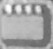
\includegraphics[width=.25\textwidth]{TemplateMatching/img/board_template_pyramid_0} &
	
\includegraphics[width=.25\textwidth]{TemplateMatching/img/board_template_pyramid_1} &
	
\includegraphics[width=.25\textwidth]{TemplateMatching/img/board_template_pyramid_2}	

	\endtabular
	\caption{Example image pyramid.}
	\label{fig:TemplatePyramid}
\end{table}

\paragraph*{}
Pyramid matching is a technique proposed\cite{Tanimoto81} by Tanimoto, that utilizes image pyramids to combine advantages of high-precision search for template occurrences in the original images with the benefits of high-speed search in the downsampled images. 

\paragraph*{}
Pyramid search commences by computing pyramids of both the input images. The height of the pyramid is a parameter of the algorithm. It should be set to maximum value for which the template is still recognizable on the highest level of its pyramid.

\paragraph*{}
Once the image pyramids are computed, the exhaustive search for template occurrences is run using significantly downsampled images on the highest pyramid level. Similar search is then repeated at successive pyramid levels down to the original images, however on each level only the template positions that scored high on the previous level are considered.

\paragraph*{}
In this way the image areas that are unlikely to contain template occurrences are pruned from the computation on the coarse level, while promising positions are pursued through every level and in the end are identified with high precision on the original images.

\subsubsection{Multi-angle Matching}

\paragraph*{}
So far we have been assuming that the template to be identified has a fixed orientation in relation to the image axes, which is rarely the case in practice. The search process that we have described has to be therefore extended to allow for rotations of the template.

\paragraph*{}
To achieve that, we will add two additional parameters to the specification of the problem instance: a range of allowed orientations and the angular precision of the search. For instance, angle range ($-15^{\circ}$, $15^{\circ}$) and angle precision $1.0^{\circ}$ would mean that $31$ rotations of the input template shall be taken into account in the search routine. For each such rotations, separate pyramid of the template image will be computed.

\paragraph*{}
In the search procedure itself we need to identify possible match candidates using tuples of $(position, rotation)$, rather than sole positions. As such extension of the pyramid search increases the computational load roughly by the factor of the number of rotations to be considered, it is advisable to limit the range of angles being considered whenever possible (e.g. when technical conditions prevent significant deviations of the template occurrences orientation). Example results obtained using this technique are presented in \reffig{MultiAngle}

\oneFigure
{TemplateMatching/img/board_graymatching_results}
{Results on the multi-angle matching of the example data.}
{MultiAngle}
{\basicWidth}

\paragraph*{}
Similar extension may be used to match the template on multiple scales, yet such need is less common than the multi-angle matching.

\subsection{Offline Phase}

\paragraph*{}
From the above description of pyramid matching it is clear that certain amount of preprocessing is required both for the template and the search image. It is important to note, that the computational load of preprocessing for these two images is \textbf{not} equally important.

\paragraph*{}
It is extremely rare to perform template matching with one-off template - usually the template is fixed and used for inspection of a whole series of images, e.g. being captured and analyzed online. The preprocessing of the template image almost always may be performed offline and as such does not need to be the focus of possible optimizations. The results of such preprocessing along with the template image are often saved in a form of atomic datatype for easy reuse.

\paragraph*{}
The preprocessing of the search image on the other hand in most cases has to be performed online and therefore its efficiency may be crucial for the feasibility of the whole template matching-based solution. It is worth noting that the extension of the pyramid matching to multiple orientations requires computing of separate pyramids of the \textbf{template image} for every possible rotation, while the preprocessing of the search image remains limited to the calculation of a single pyramid.  

\begin{refImpl}
The measures of image similarity are implemented in \studio filters:
\begin{itemize}
	\item \filter{ImageCorrelation}{ImageMetrics}, \filter{ImageCorrelationImage}{ImageMetrics}
	\item \filter{ImageDifference}{ImageMetrics}, \filter{ImageDifferenceImage}{ImageMetrics}
\end{itemize}
First filter of each pair computes a single similarity value for two images of equal dimensions, while the second filter performs a template similarity evaluation of each possible template alignment and represents the results in form of an image, as previously described.

\paragraph*{}
Brightness-based pyramid matching is implemented in three \studio filters: \filter{CreateGrayModel}{TemplateMatching}, \filter{LocateSingleObject\_NCC}{TemplateMatching} and \filter{LocateMultipleObjects\_NCC}{TemplateMatching}- first filter performs the offline, template preprocessing phase and stores the results in atomic, reusable datatype called \textit{model}, which can be later used to perform the actual matching using the second and third filter.
\end{refImpl}
\section{Edge-Based Matching}

\paragraph*{}
While the properties of normalized cross-correlation and efficiency boost offered by the pyramid matching make decent implementations of brightness-based template matching suitable for a range of typical applications, the algorithm retains a few weaknesses such as sensitivity to non-linear illumination changes and low capability of matching partially visible (occluded) template occurrences.

\paragraph*{}
As we have already noted, image edges are usually well preserved under disturbances of the illumination. Moreover, edges of an object define precisely its shape and therefore are a suitable discriminant for the identification of possible matches. The idea of edge-based template matching has been subject to extensive research and numerous measures of edge-based similarity between two images have been proposed. 

\subsection{Symmetric Methods}

\paragraph*{}
Perhaps the most fundamental classification of the edge-based template matching methods would be based on the relation between the template image and search image processing being performed by the algorithm. The earliest edge-based template matching methods were built upon edge extraction performed in the same way on both images. 

\paragraph*{}
One of the earlies methods was proposed\cite{Borgefors88} by Borgefors, who suggested to extract the edge pixels in both images and evaluate the matches using the \textbf{mean squared distance} between each edge pixel of the template image and the nearest edge pixel in the search image. 

\paragraph*{}
Rucklidge proposed\cite{Rucklidge95} a similar measure based on the \textbf{Hausdorff distance} between the edges extracted in both images, in which the difference between two images equals the maximum of two distances:
\begin{itemize}
	\item Longest distance between a template image edge pixel and any of the search image edge pixels.
	\item Longest distance between a search image edge pixel and any of the template image edge pixels.
\end{itemize}

\paragraph*{}
The major weakness of these and similar methods lies in the very idea of symmetric edge extraction. While the accurate edge extraction in the template image should not pose a problem, the assumption that the method which worked for the template image will consistently work for each search image, possibly under variable lightning conditions, is by far overoptimistic.

\paragraph*{}
Moreover, both methods are inherently sensitive to occlusions and as such have few, if any, advantages over the normalized cross-correlation grayscale-based template matching.

\subsection{Asymmetric Methods}

\paragraph*{}
To overcome the limitations of the symmetric edge-matching we need to move towards asymmetric methods. Steger proposed\cite{Steger02} to perform full edge detection in the template image, precisely identifying its contours; while each search image would be subject only to simple gradient computation on its entire area. Each possible match is then evaluated based on the correspondence of the gradient direction between the template and search image, but only at the positions of template edge pixels.

\paragraph*{}
This idea is demonstrated in \reffig{AsymetricEdges}, where we use colors from the HSV circle to represent gradient directions.

\fourFigures
{TemplateMatching/img/AssymetricEdges_template}
{TemplateMatching/img/AssymetricEdges_search}
{TemplateMatching/img/AssymetricEdges_template_edges}
{TemplateMatching/img/AssymetricEdges_search_gradient}
{Asymmetric edge processing - template image (a) is subject to full edge detection after which gradient direction at its edge pixels is computed (c), while for the corresponding section of the search image (b) computation of the gradient direction is performed indiscriminately on its entire area (d).}
{AsymetricEdges}
{.3\textwidth}

\paragraph*{}
Such approach immediately eliminates the problem of accurate edge extraction in the search image, as no such extraction is performed. Moreover, it utilizes matching of the edge directions, not only their presence, which was earlier demonstrated\cite{Olson97} by Olson et al. as advantageous in eliminating false-positive results in case of Hausdorff distance metric.

\paragraph*{}
The specific method of calculating the score of a match proposed by Steger is the simple sum of cosines of the angles between the corresponding gradient vectors, resembling the idea behind the normalized cross-correlation measure.

\paragraph*{}
Matching based on gradient direction does not preclude the application of pyramid matching schema. It is interesting to note that the asymmetric method actually outperforms the traditional grayscale-based template matching in terms of speed, as the evaluation of each possible match is limited to edge pixels of the template image; while the additional burden of computing the gradient of search image pyramid is not significant (compared with the dominating cost of the match evaluation).

\paragraph*{}
The method also works well against occlusions, as each missing edge pixel in the search image contribute at most the penalty of $-1$ to the final score, which equals in magnitude the input of a perfectly matched gradient direction, yielding cosine value of $1$. A detailed evaluation of the performance of this method is given in \cite{UlrichSteger02}.

\begin{refImpl}
Edge-based template matching is implemented in two \studio filters: \filter{CreateEdgeModel}{TemplateMatching} and \filter{MatchEdgeyModel}{TemplateMatching}.
\end{refImpl}
\section{Examples}

\subsection{Positioning of Scope Primitives}

\paragraph*{}
Template matching techniques are commonly applied to position scan lines, regions of interest, prototype shapes, etc. over an appropriate element of the object being inspected. To do so, a characteristic object location of a fixed position in relation to the area being measured is selected, and the scope primitives are defined relatively to the characteristic location.

\paragraph*{}
Then, during the actual inspection, characteristic locations of the object instances are identified using template matching techniques, and the scope primitives are positioned accordingly, as demonstrated in \reffig{Reposition}.

\twoFigures
{TemplateMatching/img/Reposition_model}
{TemplateMatching/img/Reposition_results}
{Template matching used for alignment of the scan lines for \refchap{1DEdgeDetection}.}
{Reposition}
{\basicWidth}





\include{_ConcludingRemarks}

%\backmatter 
%\include{glossary} 
%\include{notat} 
\bibliographystyle{unsrt}
\bibliography{bibliography}
\printindex

\end{document} 